\documentclass[prodmode,acmtcps]{acmsmall}

% Metadata Information
\acmVolume{9}
\acmNumber{4}
\acmArticle{39}
\acmYear{2016}
\acmMonth{7}

\usepackage{graphicx}
%\graphicspath{{figs/}}
\usepackage{paralist}
\usepackage{todonotes}  %\newcommand{\todo}[][a]{}
\usepackage{color}
\usepackage{epstopdf}
\usepackage{subfigure}
\usepackage{amssymb}
\usepackage{amsfonts}
\usepackage{cool}  % COntext-Oriented math for LaTeX
\usepackage{mleftright}  % Commands \mleft and \mright
\usepackage{booktabs}
%\usepackage{subfloat}
\usepackage[per-mode=symbol]{siunitx}
\usepackage{url}

\usepackage{hyperref}
\hypersetup{citecolor=blue, colorlinks=true}
\usepackage[font=small]{caption}
\usepackage{cite}

% Also, note that the amsmath package sets \interdisplaylinepenalty to 10000
% thus preventing page breaks from occurring within multiline equations. Use:
%\interdisplaylinepenalty=2500
% after loading amsmath to restore such page breaks

\usepackage[amsmath,thmmarks,thref]{ntheorem}
\usepackage{algorithm,algpseudocode}
\theoremstyle{definition}
\newtheorem{observation}{Observation}
\usepackage{truonglatexdefs}

\usepackage{enumitem, kantlipsum}
\usepackage{tikz}
\usetikzlibrary{arrows}
\tikzset{
  treenode/.style = {align=center, inner sep=0pt, text centered},
  branch_c/.style = {treenode, circle, black, draw=black,
    text width=1.5em, very thick},  
  branch_l/.style = {treenode, circle, blue!50!gray!, draw=blue!50!gray!,
    text width=1.5em, very thick},
  branch_r/.style = {treenode, circle, red!50!gray!, draw=red!50!gray!, 
    text width=1.5em, very thick},
}

%\newcommand{\tableref}[1]{Table~\ref{tab:#1}}
%\newcommand{\figref}[1]{Fig.~\ref{fig:#1}}
%\newcommand{\listref}[1]{Listing~\ref{list:#1}}
% Clever references -- SHOULD BE LOADED LAST
% Generic commands: \cref and \Cref
% Seems incompatible with `algorithmic' from algorithms bundle, but can be used with `algorithmicx' (e.g. `algpseudocode').
%\usepackage[capitalise]{cleveref}
%\newcommand{\vref}[1]{\cref{#1}}
% When using \namecref, cleveref capitalizes the first character if the option capitalise is used, which I don't want.  So use \lcnamecref instead.

%\setlength{\textheight}{9.65in}
\setlength{\textwidth}{6.4in}
%\setlength{\columnsep}{0.3125in}
%\setlength{\topmargin}{-.25in}
%\setlength{\headheight}{-.1in}
%\setlength{\headsep}{0in}
%\setlength{\parskip}{0cm}
%\setlength{\parindent}{1pc}
%\setlength{\partopsep}{0pt}
\setlength{\oddsidemargin}{-.005in}
\setlength{\evensidemargin}{-.005in}
%
%\setlength{\abovedisplayskip}{0pt}
%\setlength{\belowdisplayskip}{0pt}
%\setlength{\abovedisplayshortskip}{0pt}
%\setlength{\belowdisplayshortskip}{0pt}

\linespread{0.96}
%\usepackage{balance}


%\usepackage{etoolbox}
%\makeatletter
%\patchcmd{\maketitle}{\@copyrightspace}{}{}{}
%\makeatother

%\apptocmd{\thebibliography}{\small}{}{}

\begin{document}
% Page heads
\markboth{A. Jain et al.}{Data Predictive Control for Cyber-Physical Energy Systems}

% Title portion
\title{Data Predictive Control for Cyber-Physical Energy Systems}
\author{ACHIN JAIN
\affil{University of Pennsylvania}
MADHUR BEHL
\affil{University of Virginia}
RAHUL MANGHARAM
\affil{University of Pennsylvania}}

% NOTE! Affiliations placed here should be for the institution where the
%       BULK of the research was done. If the author has gone to a new
%       institution, before publication, the (above) affiliation should NOT be changed.
%       The authors 'current' address may be given in the "Author's addresses:" block (below).
%       So for example, Mr. Abdelzaher, the bulk of the research was done at UIUC, and he is
%       currently affiliated with NASA.

\begin{abstract}


Decisions on how best to optimize today's energy systems operations are becoming ever so complex and conflicting such that model-based predictive control algorithms must play a key role. However, learning dynamical models of energy consuming systems such as buildings, using grey/white box approaches is very cost and time prohibitive.
Demand response (DR) is becoming increasingly important as the volatility on the grid continues to increase.
%Current DR approaches are completely manual and rule-based or involve deriving first principles based models which are extremely cost and time prohibitive to build.
We consider the problem of data-driven end-user demand response and peak power reduction for large buildings which involves predicting the demand response baseline, evaluating fixed rule based DR strategies, synthesizing DR control actions, and reducing the peak power consumption.
We provide a model based control with regression trees algorithm (mbCRT), which allows us to perform closed-loop control for DR strategy synthesis for large commercial buildings. Our data-driven control synthesis algorithm outperforms rule-based DR by 17\% for a large DoE commercial reference building and leads to a curtailment of $380\si{\kilo\watt}$ and over \$45,000 in DR revenue.
A data predictive control with regression trees (DPCRT) algorithm, is also presented. DPCRT is a finite receding horizon method, using which the building operator can optimally trade off peak power reduction against thermal comfort without having to learn white/grey box models of the systems dynamics. 
Our methods have been integrated into an open source tool called DR-Advisor, which acts as a recommender system for the building's facilities manager and provides suitable control actions to meet the desired load curtailment while maintaining operations and maximizing the economic reward. DR-Advisor achieves 92.8\% to 98.9\% prediction accuracy for 8 buildings on Penn's campus. We compare DR-Advisor with other data driven methods and rank $2^{nd}$ on ASHRAE's benchmarking data-set for energy prediction.
\end{abstract}


%
% The code below should be generated by the tool at
% http://dl.acm.org/ccs.cfm
% Please copy and paste the code instead of the example below. 
%
\begin{CCSXML}
<ccs2012>
<concept>
<concept_id>10010147.10010257.10010293.10003660</concept_id>
<concept_desc>Computing methodologies~Classification and regression trees</concept_desc>
<concept_significance>500</concept_significance>
</concept>
</ccs2012>
\end{CCSXML}

\ccsdesc[500]{Computing methodologies~Classification and regression trees}


%
% End generated code
%

% We no longer use \terms command
%\terms{Design, Algorithms, Performance}

\keywords{Machine learning; Predictive control; Cyber-physical Systems; Demand response; Peak power reduction}

\acmformat{Achin Jain, Madhur Behl and Rahul Mangharam, 2016. Data Predictive Control for Cyber-Physical Energy Systems.}

% At a minimum you need to supply the author names, year and a title.
% IMPORTANT:
% Full first names whenever they are known, surname last, followed by a period.
% In the case of two authors, 'and' is placed between them.
% In the case of three or more authors, the serial comma is used, that is, all author names
% except the last one but including the penultimate author's name are followed by a comma,
% and then 'and' is placed before the final author's name.
% If only first and middle initials are known, then each initial
% is followed by a period and they are separated by a space.
% The remaining information (journal title, volume, article number, date, etc.) is 'auto-generated'.

\begin{bottomstuff}
Author's addresses: {A. Jain {and} R. Mangharam, Department of Electrical and Systems Engineering,
University of Pennsylvania; M. Behl,
Department of Computer Science, University of Virginia.}
\end{bottomstuff}

\maketitle

\section{Introduction}
\label{sec:intro}
2016 was the hottest year on record since the beginning of weather recording in 1880~\cite{noaa}. Heat waves in summer and polar vortexes in winter are growing longer and pose increasing challenges to an already over-stressed electric grid. Furthermore, with the increasing penetration of renewable generation, the electricity grid is also experiencing a shift from predictable and dispatchable electricity generation to variable and non-dispatchable generation. This adds another level of uncertainty and volatility to the electricity grid. The volatility due to the mismatch between electricity generation and supply further leads to volatility in the wholesale price of electricity. For example, the polar vortex triggered extreme weather events in the U.S. in January 2014, which caused many electricity customers to experience increased costs. Parts of the U.S. north-eastern electricity grid experienced a 86-fold increase in the price of electricity from $\$31/\si{\mega\watt\hour}$ to $\$2,680/\si{\mega\watt\hour}$ in a matter of a few minutes~\cite{volatility}.  Such events show how unforeseen and uncontrollable circumstances can greatly affect electricity prices that impact grid operator and customers. Electricity price volatility, is becoming the new norm rather than the exception.

Across the United States, utilities and grid operators are devoting increasing attention and resources to Demand Response (DR). It is considered as a reliable means of mitigating the uncertainty and volatility of renewable generation and extreme weather conditions and improving the grid's efficiency and reliability. The resource contribution from all U.S. DR programs is estimated to be nearly 72,000 MW, or about 9.2 percent of U.S. peak demand~\cite{federal2008assessment} making DR the largest virtual generator in the U.S. national grid. The annual revenue to end-users from DR markets with PJM ISO alone is more than \$700 million~\cite{pjm}. Global DR revenue is expected to reach nearly \$40 billion from 2014 through 2023~\cite{navigant}.

The volatility in real-time electricity prices poses the biggest operational and financial risk for large scale end-users of electricity such as large commercial buildings, industrial and institutional customers (often referred to as \textit{C/I/I} consumers). In order to shield themselves from the volatility and risk of high prices, such consumers must be more flexible in their electricity demand. Consequently, large \textit{C/I/I} customers are increasingly looking to demand response programs to help manage their electricity costs. DR programs involve a voluntary response of a building to a price signal or a load curtailment request from the utility or the Curtailment Service Provider (CSP). Upon successfully meeting the required curtailment level the end-users are financially rewarded, but may also incur penalties for under-performing and not meeting a required level of load curtailment. In practice, one of the biggest challenges with end-user demand response is the following: \emph{Upon receiving the notification for a DR event, what actions must the end-user take in order to achieve an adequate and a sustained DR curtailment?} 

Unfortunately, most of the Demand Response today is done in an ad-hoc manner. 
The decisions are rule-based or they depend upon a building operator's experience, which has several disadvantages:

\begin{itemize}[leftmargin=0.5cm]
	\item \emph{Limitations of rule-based DR:} The building's operating conditions, internal thermal disturbances and environmental conditions must all be taken into account to make appropriate DR control decisions, which is not possible with using rule-based and pre-determined DR strategies since they do not account for the state of the building but are instead based on best practices and rules of thumb. 
	Rule based DR strategies have the advantage of being simple but they do not account for the state of the building and weather conditions during a DR event.
	\item \emph{Control complexity and scalability.} Upon receiving a notification for a DR event, the building's facilities manager must determine an appropriate DR strategy to achieve the required load curtailment. 
	These control strategies can include adjusting zone temperature set-points, supply air temperature and chilled water temperature set-point, dimming or turning off lights, decreasing duct static pressure set-points and restricting the supply fan operation \etc
	In a large building, it is difficult to assess the effect of one control action on other sub-systems and on the building's overall power consumption because the building sub-systems are tightly coupled.
\end{itemize}
These drawbacks are addressed by predictive control techniques such as Model Predictive Control (MPC). MPC allows to optimize desired performance while guaranteeing system's constraints. For example, it can be used to provide the optimal actions for an energy curtailment during a DR event while guaranteeing thermal comfort for occupants. So MPC-based solutions fit into the DR problem. However, the quality of the MPC solutions depends on the accuracy of the predictive models describing the system. This limits the widespread of MPC for complex systems such as buildings. Thus, in context of modeling of large buildings, applying MPC poses further challenges:

\begin{itemize}[leftmargin=0.5cm]
\item \emph{Modeling complexity and heterogeneity.} Unlike the automobile or the aircraft industry, each building is designed and used in a different way and therefore it must be uniquely modeled. Learning predictive models of building's dynamics using first principles based approaches (\eg with EnergyPlus~\cite{Crawley2001319}) is very cost and time prohibitive and requires retrofitting the building with several sensors~\cite{costmpc}. The user expertise, time and costs required to develop a model of a single building are very high.
%\item \emph{Interpretability of modeling and control.} Predictive models for buildings, regardless how sophisticated, lose their effectiveness unless they can be interpreted by human experts and facilities managers in the field. Therefore, the required solution must be transparent, human centric and highly interpretable.
\end{itemize}

\subsection{Main contribution}

In order to address the aforementioned challenges, we use machine learning algorithms to generate data-driven models for cyber-physical systems where we preserve predictive capability of model-based control but without the expense of first principle or grey-box model development.
Although machine learning algorithms are a popular choice for predicting systems' behavior, they do not provide models that are suitable for control.
In our previous work \cite{BehlJainMangharam2016,Behl201630}, we overcome this issue by using regression tree-based algorithms to provide models of system dynamics to be used in an optimal control problem setup.
%We  discussed the use of regression trees-based approaches to estimate the DR baseline power consumption and to build auto-regressive trees for DR control strategies evaluation.
%We further showed the procedure to design such a controller for energy management during Demand Response.
We proposed an algorithm for model-based control using regression trees (mbCRT), and apply it to synthesize real-time DR strategy.
The mbCRT algorithm can be used to setup optimal control problems with one-step lookahead prediction, for example to trade off thermal comfort inside a building against the amount of load curtailment.
However, mbCRT cannot be used to setup a receding horizon control problem with an arbitrarily length of the horizon as in MPC. 
This drawback limits the closed-loop control performance since it does not take into account the very accurate long term state prediction that regression trees can provide. 
In this paper, we overcome this issue providing the following contributions:

\begin{itemize}[leftmargin=0.5cm]
	\item \emph{Multi-variate regression trees:} We introduce a methodology to construct a multi-variate or multi-output predictive model using regression trees, where each output corresponds to the prediction on a future step of the horizon. More precisely, we setup a least square problem that minimize the prediction error over the control horizon. This is done by modifying the variable selection and splitting criteria at the nodes of the standard regression tree algorithm CART \cite{BreimanFriedmanStoneEtAl1984}.
	\item \emph{Predictive control:} We extend the mbCRT algorithm proposing a Data-driven Predictive Control strategy using Regression Trees (DPCRT), that implements receding horizon control using data-based models learned from the available historical data.
	\item \emph{Application:} We apply this control strategy to peak power curtailment on a large office building and compare with the previous mbCRT algorithm. Our results show an improvement of $8.6\%$ in terms of peak curtailment is obtained using DPCRT with respect to mbCRT.
\end{itemize}
In summary, the methodology proposed in this paper bypasses the cost and time prohibitive process of building high fidelity models (using grey and white box approaches) while still being suitable for receding horizon control. 
%These are the first algorithms of its kind that enable closed-loop control synthesis and finite receding horizon control with regression trees. 
The contributions of the paper are graphically shown in Fig. \ref{F:scheme}.

\subsection{Related work}
\label{sec:related}
In recent years, data-driven optimal control has drawn a huge interest in the research community.
Several different approaches have been considered. 
For example, in one approach, models are trained on optimal solutions obtained from MPC. 
The resulting models can then be used for explicit MPC, as in~\cite{BemporadMorariDuaEtAl2002}. This approach has been applied to problems of stabilization \cite{CavagnariMagniScattolini1999} and freeway traffic systems using regression trees \cite{OleariFrejoCamachoEtAl2015}. 
In applications like buildings, where obtaining a model for MPC is hard, such techniques cannot be used.
Another class of methods solve the optimization directly on the trained models to do predictive control \cite{Hou2013,Costanzo2016,FerreiraRuanoSilvaEtAl2012}. 
However, none of them addresses the problem of including data-driven state models into the optimal predictive control loop. Hence, we cannot solve an MPC-like optimal control problem. 
In \cite{Behl201630}, we proposed MPC-like control problem considering regression tree-based algorithms for the DR problem. In \cite{KusiakSongZheng2009}, neural networks are used instead to setup an MPC-like control for the wind turbine problem using evolutionary algorithms. Nevertheless, their approaches considered only one-step lookahead predictive model, and hence does not allow predictive control over an arbitrary horizon.

There is a vast literature more specific to the Demand Response which look at the problem of determining DR strategies \cite{oldewurtel2013towards,xu2004peak}. 
The majority of the approaches are either rule-based techniques for curtailment or white/grey box model-based control. 
These usually assume that the model of the system is well known whereas the task is much more complicated and time consuming in the case of a real building and sometimes, it can be even more complex and involved than the design of the controller itself. 
After several years of work on using first principles based models for demand response, multiple authors~\cite{costmpc,reallife} have concluded that the biggest hurdle to mass adoption of intelligent building control is the cost and effort required to capture accurate dynamical models of the buildings. 
There are ongoing efforts to make tuning and identifying white box models of buildings more autonomous~\cite{new2012autotune}. 
OpenADR standard and protocol~\cite{openadr} describes the formats for information exchange to facilitate DR but modeling, prediction and control strategies are out of scope. 
Several machine learning approaches~\cite{edwards2012predicting,vaghefi2014modeling,yin2012scalable} have been utilized before for forecasting electricity load including some which use regression trees. 
However, there are two significant shortcomings of the work in this area: 
	\begin{inparaenum}[(a)]
		\item these approaches are coarse grained and  are not aimed at solving demand response problems but are restricted to long term load forecasting with applications in evaluating building retrofits savings and building energy ratings, and
		\item  there is no focus on control synthesis or addressing the suitability of the model to be used in control design. 
	\end{inparaenum}
	There exist several different approaches to balance the power consumption in buildings and avoid peaks, e.g. by load shifting and load shedding \cite{KiliccoteEtAl06aca,LeeEtAl08dom}. However, they operate on coarse grained time scales and do not guarantee any thermal comfort.

\begin{figure}[t!]
	\begin{center}
		\hspace{0.8cm}
		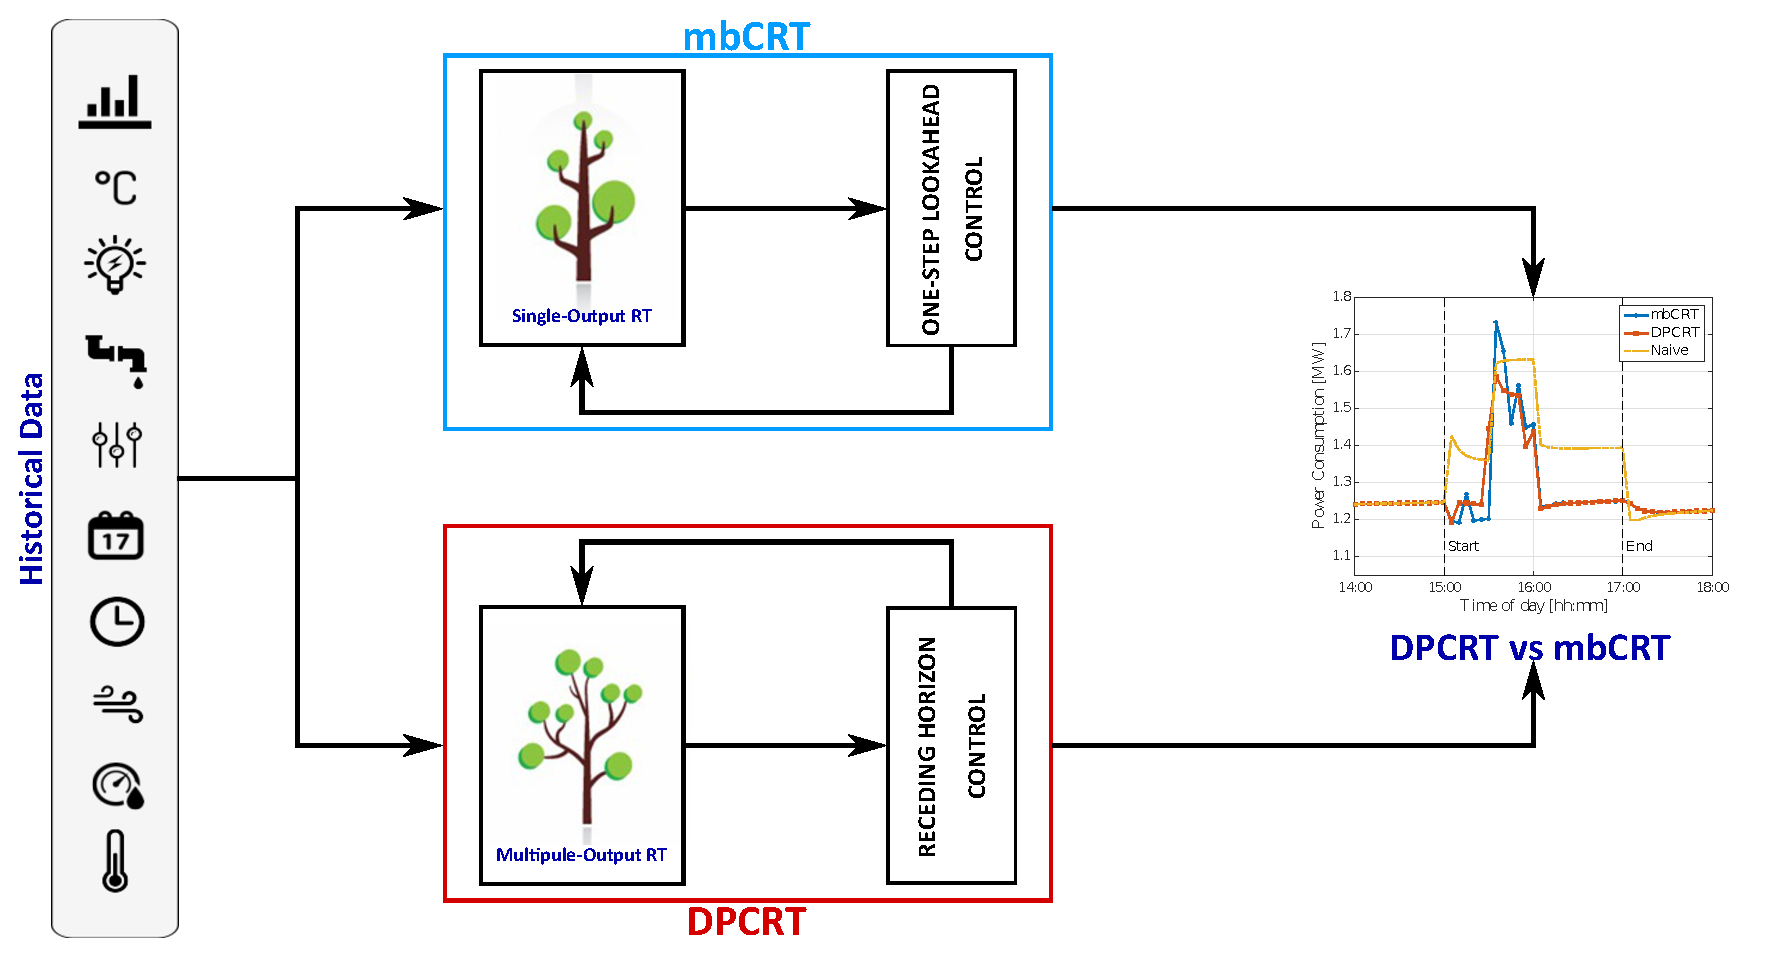
\includegraphics[width=0.8\textwidth]{Figures/scheme.eps}
		\centering
		\caption{Historical data are used to train models for mbCRT in Sec.~\ref{sec:drtree} and DPCRT in Sec.~\ref{sec:decision_tree}. These models are then used in the optimization in a closed-loop with the physical system. Finally, the two approaches are compared in Sec~\ref{sec:case}.}
		\label{F:scheme}
		\vspace{-10pt}
	\end{center}
\end{figure}

The DPCRT algorithm is first of its kind that does finite receding horizon control with regression trees. 
It is computationally efficient because the optimization problem is convex and the number of constraints scales linearly with the number of control variables. 
A preliminary version of this paper can be found in the conference paper \cite{JainBuildsys2016}.

\subsection{Paper organization}

This paper is organized as follows. We describe our problem formulation in Sec.~\ref{sec:problem}. 
Sec.~\ref{sec:drtree} provides an overview of the data-driven control strategy (mbCRT) proposed in \cite{Behl201630} that will be useful to introduce our new methodology. 
In Sec.~\ref{sec:decision_tree}, we present our main contribution -- predictive control using multi-variate regression trees. 
In particular, we extend the standard training algorithm for regression trees in Sec. \ref{SS:training_algo} so we can use it to build predictive models over a horizon of arbitrary length. 
In Sec. \ref{SS:control_tree}, we use the DPCRT algorithm to formally build system models and setup a receding horizon optimal control problem that can be used for the closed-loop control. 
Finally, in Sec. \ref{sec:case} we apply DPCRT to a peak power reduction problem and compare it with mbCRT.



\section{Problem Definition}
\label{sec:problem}
\textcolor[rgb]{0.00,0.00,1.00}{Our goal is to find data-driven functional models for cyber-physical systems starting from available historical data. The aim is to build models that relate the value of the response variables $\mathrm{y}_1,\ldots,\mathrm{y}_p$ with the values of the predictor variables or features $\mathrm{x}_1,\ldots,\mathrm{x}_s$, and that can be used to setup an optimization predictive control problem. For example, in the case of buildings the response variables can be represented by the power consumption or the room temperatures, while the features can be represented by weather data, set-points information and building schedules.}
\textcolor[rgb]{1.00,0.00,0.00}{When the dataset has lots of features, as in the case of large buildings, which interact in complicated nonlinear ways, assembling a single global model, such as linear or polynomial regression, can be difficult and lead to poor response predictions. An approach to non-linear regression is to partition the data space into smaller regions $R_i$, where the interactions are more manageable. Regression trees are an example of an algorithm which belongs to the class of recursive partitioning algorithms. The seminal algorithm for learning regression trees is CART as described in~\cite{BreimanFriedmanStoneEtAl1984}. Regression trees-based approaches are our choice to construct data-driven models for cyber-physical systems. The primary reason for this modeling choice is that regression trees are highly interpretable by design. Interpretability is a fundamental desirable quality in any predictive model. Complex predictive models like neural networks, support vector regression \etc go through a long calculation routine and involve too many factors. It is not easy for a human engineer to judge if the operation/decision is correct or not or how it was generated in the first place. For example, building operators are used to operating a system with fixed logic and rules. They tend to prefer models that are more transparent, where it is clear exactly which factors were used to make a particular prediction. At each node of a regression tree, a simple "if this then that" human readable plain text rule is applied to generate a prediction at the leafs, which anyone can easily understand and interpret. Making machine learning algorithms more interpretable is an active area of research, one that is essential for incorporating human centric models in cyber-physical systems.}

\textcolor[rgb]{0.00,0.00,1.00}{We want to use such regression trees-based models to setup optimal predictive control strategies as in the classical MPC formulation. The main problem rising up when dealing with machine learning algorithms is that they do not provide mathematical models that are directly usable for control. To overcome this issue we propose a solution that is based on the \emph{separation of variables}. In particular, given a dataset $(\mathcal{X},\mathcal{Y})$, where $\mathcal{X}=\{\x_1,\ldots,\x_s\}$ is the set of predictor variables (or features) and $\mathcal{Y}=\{\y_1,\ldots,\y_p\}$ is of response variables, we want to use regression trees to learn a model $f_i$ to predict the response $\y_i$ as }
\textcolor[rgb]{0.00,0.00,1.00}{
\begin{equation}\label{eq:RTmodel}
	\y_i=f_i(\x_1,\ldots,\x_s)
\end{equation}
}

\textcolor[rgb]{0.00,0.00,1.00}{
Given a forecast of predictor variables $\hat{\x}_i$, we can predict system response using \eqref{eq:RTmodel}. However, suppose the set of system inputs $\mathcal{X}_c$, that are the variables we can manipulate is a subset of the features set, i.e. $\mathcal{X}_c=\{\mathrm{u}_1,\ldots,\mathrm{u}_m\}\subset\mathcal{X}$. Suppose we want to setup a receding horizon control problem to find optimal inputs that optimize a performance cost function. Let $u(t)=[\mathrm{u}_1(t),\ldots,\mathrm{u}_m(t)]$ be the vector of inputs applied to the system at time $t$ to be optimized, $x(t) = [\mathrm{x}_1(t),\ldots,\mathrm{x}_{s-m}(t)]$ be the vector of system variables measured at time $t$, and $y(t) = [\mathrm{y}_1(t),\ldots,\mathrm{y}_{p}(t)]$ be the vector of system response variables at time $t$, then model \eqref{eq:RTmodel} can not be used to solve the following optimal predictive control problem}

\textcolor[rgb]{0.00,0.00,1.00}{
\begin{equation}\label{eq:linear_program}
\begin{aligned}
& \underset{u_{t+k}\in\mathcal{X}_c}{\text{minimize}} & &  \sum_{k = 0}^{N}{J(y_{t+k},u_{t+k})}  \\
& \text{subject to }                                  & &  y_{t+k}    =   f(x_{t+k},u_{t+k})     \\
&                                                     & &  u_{t+k}   \in \mathcal{\bar U}        \\
&                                                     & &  y_{t+k}   \in \mathcal{\bar Y}        \\
&                                                     & &  x_{t}      =   x(t)                   \\
&                                                     & &  k          =   0,\ldots,N             \\
\end{aligned}
\end{equation}
This is because inputs $u$ are optimization variables, hence they are not known a priori to be used as features to build the prediction using \eqref{eq:RTmodel}.}

\textcolor[rgb]{0.00,0.00,1.00}{
\emph{Separation of variables} is a technique that consists on partitioning the features dataset into inputs (or control variables) and disturbances sets, i.e. the sets of variables we can and can not manipulate, respectively. More precisely, $\mathcal{X} = \mathcal{X}_c\biguplus\mathcal{X}_d$, where $\biguplus$ represents the disjoint union. The regression tree is trained only using the disturbance variables in $\mathcal{X}_d$, so that we can associate to each leaf a model that depends only on the inputs data. In this way we can use disturbances forecasts to predict the system behavior using \eqref{eq:RTmodel}. This procedure provides a modeling framework that allows to solve optimization problem \eqref{eq:linear_program}. In the next $2$ sections we show how this is achieved. In particular, in the next section we recall the mbCRT algorithm, that uses separation of variables to create a regression trees-based model that can be used to solve optimization problem \eqref{eq:linear_program} for the one step lookahead case, i.e. only with $N=0$. Then we provide a novel methodology, based on the redefinition of the regression trees learning algorithm, so that optimization problem \eqref{eq:RTmodel} can be solved for arbitrary $N$. We finally compare in Sec. \ref{sec:case} the performance of the $2$ approaches to show how the long term prediction can improve system performance.}


%\section{Learning regression trees}
%\label{sec:rtree}
%\input{trees.tex}

\section{Data-Driven Demand Response}
\label{sec:drtree}
Our goal is to find data-driven functional models that relates the value of the response variable $\mathbb{Y}$, say power consumption $\mathcal{P}$, with the values of the predictor variables or features $\left[ \mathbb{X}^1,\dots,\mathbb{X}^n \right]$ which can include weather data, set-point information and building schedules.
When the data has lots of features, as is the case in large buildings, which interact in complicated, nonlinear ways, assembling a single global model, such as linear or polynomial regression, can be difficult, and lead to poor response predictions.
An approach to non-linear regression is to partition the data space into smaller regions, where the interactions are more manageable. 
% We then partition the partitions again; this is called recursive partitioning, until finally we get to chunks of the data space which are so tame that we can fit simple models to them. 
%Therefore, the global model has two parts: the recursive partition, and a simple model for each cell of the partition.
Regression trees is an example of an algorithm which belongs to the class of recursive partitioning algorithms. The seminal algorithm for learning regression trees is CART as described in~\cite{breiman1984classification}. 

Regression trees based approaches are our choice of data-driven models for DR-Advisor. The primary reason for this modeling choice is that regression trees are highly interpretable, by design.
Interpretability is a fundamental desirable quality in any predictive model.  
Complex predictive models like neural-networks , support vector regression \etc go through a long calculation routine and involve too many factors. 
It is not easy for a human engineer to judge if the operation/decision is correct or not or how it was generated in the first place. 
Building operators are used to operating a system with fixed logic and rules. 
They tend to prefer models that are more transparent, where it is clear exactly which factors were used to make a particular prediction.
At each node in a regression tree a simple, if this then that, human readable, plain text rule is applied to generate a prediction at the leafs, which anyone can easily understand and interpret.
%Making machine learning algorithms more interpretable is an active area of research~\cite{giraud1998beyond}, one that is essential for incorporating human centric models in cyber-physical energy systems.
Making machine learning algorithms more interpretable is an active area of research, one that is essential for incorporating human centric models in cyber-physical energy systems.

\subsection{Data-Description}

In order to build regression trees which can predict the power consumption of the building, we need to train on time-stamped historical data. As shown in Fig.~\ref{fig:overview}, the data that we use can be divided into four different categories as described below:
\begin{enumerate}
\item \textbf{Weather Data $\mathcal{W}$:} This includes measurements of the outside dry-bulb and wet-bulb air temperature, relative humidity, and wind characteristics. Since we are interested in predicting the power consumption for a finite horizon, we include the weather forecast of the complete horizon in the training features.
\item \textbf{Schedule Data $\mathcal{S}$:} We create proxy variables which correlate with repeated patterns of electricity consumption e.g., due to occupancy or equipment schedules. Day of Week is a categorical predictor which takes values from 1-7 depending on the day of the week. This variable can capture any power consumption patterns which occur on specific days of the week. Likewise, Time of Day is quite an important predictor of power consumption as it can adequately capture daily patterns of occupancy, lighting and appliance use without directly measuring any one of them. Besides using proxy schedule predictors, actual building equipment schedules can also be used as training data for building the trees.
\item \textbf{Building Data $\mathcal{B}$:} The state of the building includes (i) Chilled Water Supply Temperature, (ii) Hot Water Supply Temperature, (iii) Zone Air Temperature, (iv) Supply Air Temperature, and (v) Lighting levels.
\item \textbf{Power Consumption $\mathcal{P}$:} This is the response variable, in addition to zone temperatures. We also considered autoregressive terms of power consumption in the input. 
An auto-regressive tree model is a regular regression tree except that the lagged values of the response variable are also predictor variables for the regression tree.
\end{enumerate}

\subsection{Data-Driven DR Baseline}

DR-Advisor uses a mix of several algorithms to learn a reliable baseline prediction model. For each algorithm, we train the model on historical power consumption data and then validate the predictive capability of the model against a test data-set which the model has never seen before.
In addition to building a single regression tree, we also learn cross-validated regression trees, boosted regression trees (BRT) and random forests (RF). The ensemble methods like BRT and RF help in reducing any over-fitting over the training data. They achieve this by combining the predictions of several base estimators built with a given learning algorithm in order to improve generalizability and robustness over a single estimator.
For a more comprehensive review of random forests we refer the reader to~\cite{breiman2001random} and to~\cite{elith2008working} for an explanation of boosted trees.

\subsection{Data-Driven DR Evaluation}
\label{sec:autort}

The regression tree models for DR evaluation are similar to the models used for DR baseline estimation except for two key differences:
First, instead of only using weather and proxy variables as the training features, in DR evaluation, we also train on set-point schedules and data from the building itself to capture the influence of the state of the building on its power consumption; and 
Second, in order to predict the power consumption of the building for the entire length of the DR event, we use the notion of auto-regressive trees. An auto-regressive tree model is a regular regression tree except that the lagged values of the response variable are also predictor variables for the regression tree \ie the tree structure is learned to approximate the following function:
%\begin{equation}
%\hat{Y_{kW}(t)} = f([X_1, X_2,\cdots, X_m,Y_{kW}(t-1),\cdots,Y_{kW}(t-\delta)])
%\end{equation}
\begin{gather}
  \mathcal{P}(t) = \mathit{f} \left( \mathcal{W}(t), \mathcal{S}(t), \mathcal{B}(t), \mathcal{P}(t-1),\dots, \mathcal{P}(t-\delta) \right).
\label{E:building_model}
\end{gather}
where the predicted power consumption response $\mathcal{P}$ at time $t$, depends on previous values of the response itself $ \mathcal{P}(t-1),\dots, \mathcal{P}(t-\delta)$ and $\delta$ is the order of the auto-regression.
This allows us to make finite horizon predictions of power consumption for the building.
At the beginning of the DR event we use the auto-regressive tree for predicting the response of the building due to each rule-based strategy and choose the one which performs the best over the predicted horizon. The prediction and strategy evaluation is re-computed periodically throughout the event.

\section{Data-Driven Control Synthesis}
\label{sec:drsyn}
The data-driven methods described so far use the forecast of features to obtain building power consumption predictions  for DR baseline and DR strategy evaluation.
In this section, we extend the theory of regression trees to solve the demand response synthesis problem described earlier in Sec.~\ref{sec:synthesis}. This is one of our primary contribution.

\begin{figure}
\centering
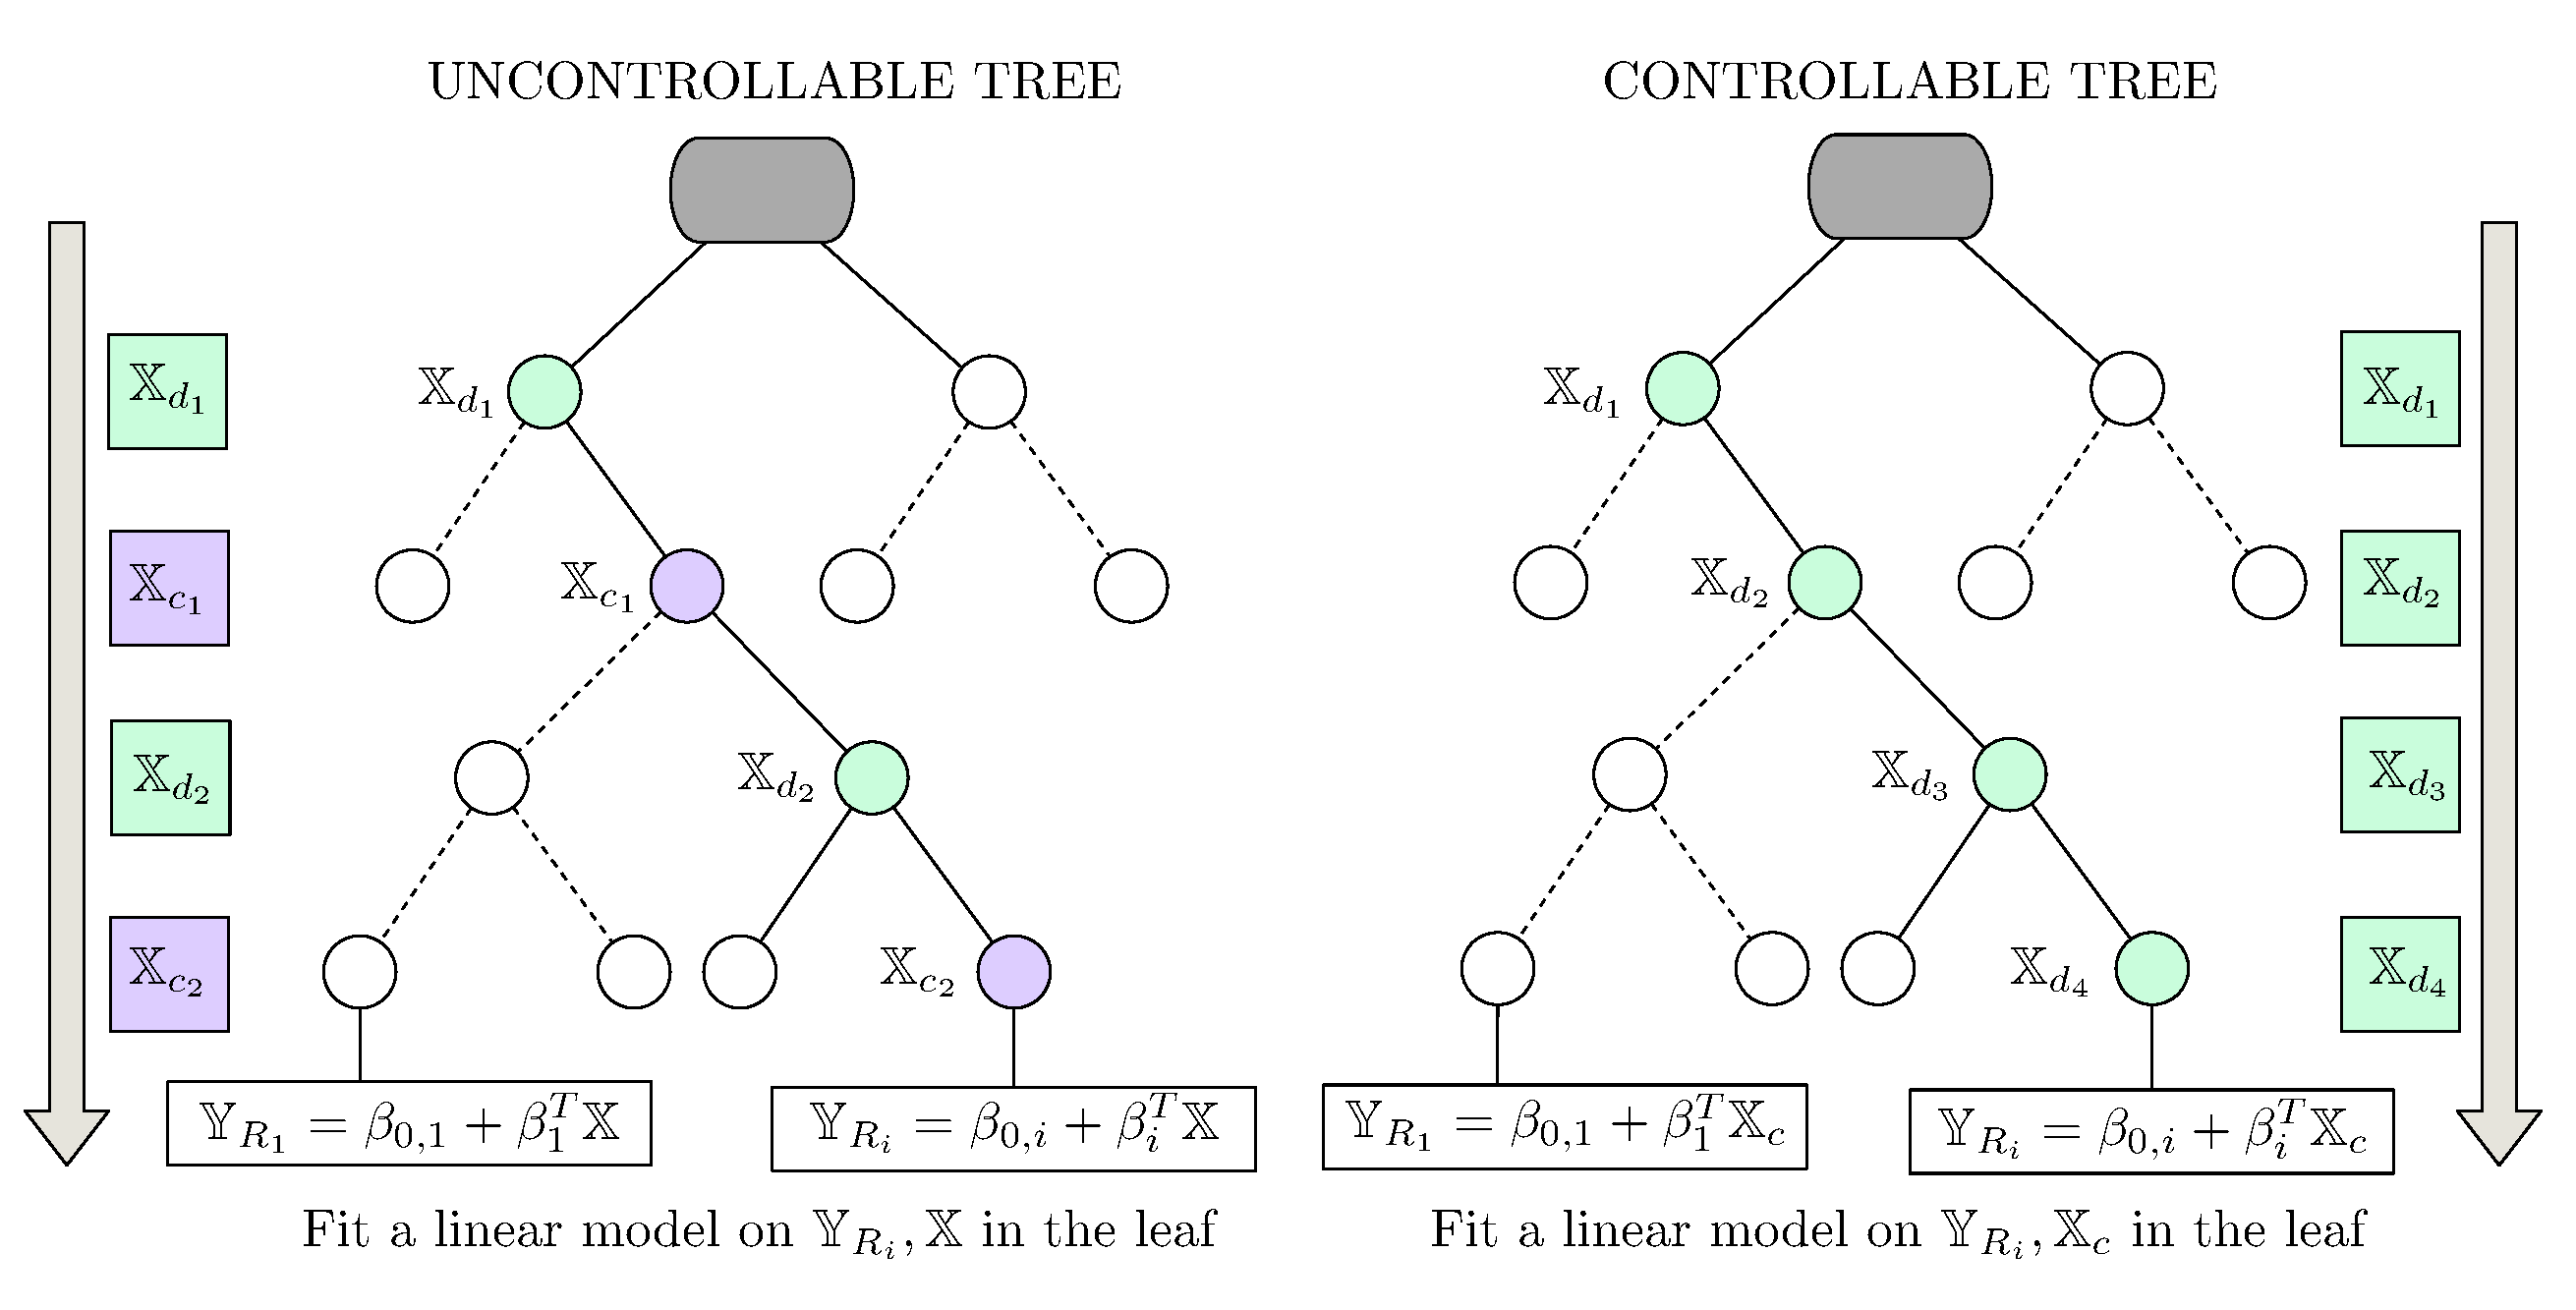
\includegraphics[width=0.95\columnwidth]{Figures/sep_vars.eps}
   \caption{Left: Example of a regression tree not suitable for control due to the mixed order of the controllable $\mathbb{X}_c$ and uncontrollable $\mathbb{X}_d$ features. Right: Example of a tree structure obtained used for mbCRT algorithm. The separation of variables allows using the linear model in the leaf to use only control variables.}
   \captionsetup{justification=centering}
   \label{fig:training}
\end{figure}
%\begin{figure*}
%\centering
%\begin{subfigure}
%  \centering
%  \includegraphics[width=0.4\columnwidth]{figs/mixed_order}
%  \end{subfigure}  
%  \begin{subfigure}
%    \centering
%  \includegraphics[width=0.5\columnwidth]{figs/sepofv-compressed}
%  \end{subfigure}
%   \caption{Left: Example of a regression tree not suitable for control due to the mixed order of the controllable $X_c$ (solid blue) and uncontrollable $X_d$ features. Right: Example of a tree structure obtained used for mbCRT algorithm. The separation of variables allows using the linear model in the leaf to use only control variables.}
%   \captionsetup{justification=centering}
%   \label{fig:training}
%\end{figure*}

Recall that the objective of learning a regression tree is to learn a model $f$ for predicting the response $\mathbb{Y}$ with the values of the predictor variables or features $\mathbb{X}^1, \dots, \mathbb{X}^n$; i.e. $\mathbb{Y}=f(\mathbb{X}^1, \dots, \mathbb{X}^n)$.
Given a forecast of the features $\hat{X}^1, \dots, \hat{X}^n$, we can predict the response $\hat{Y}$. 
Now consider the case where a subset, $\mathbb{X}_c \subset \mathbb{X}$ of the set of features/variables $\mathbb{X}$'s are manipulated variables i.e. we can change their values in order to drive the response $\mathbb{Y}$ towards a certain value. 
In the case of buildings, the set of  variables can be separated into disturbances (or non-manipulated) variables like outside air temperature, humidity, wind etc. while the controllable (or manipulated) variables would be the temperature and lighting set-points within the building.
Our goal is to modify the regression trees and make them suitable for synthesizing the optimal values of the control variables in real-time.

\subsection{Model-based control with regression trees}
\label{sec:mbcrt}

The key idea in enabling control synthesis for regression trees is in the separation of features/variables into manipulated and non-manipulated features. 
Let $\mathbb{X}_c \subset \mathbb{X}$ denote the set of manipulated variables and $\mathbb{X}_d \subset \mathbb{X}$ denote the set of disturbances/ non-manipulated variables such that $\mathbb{X}_c \cup \mathbb{X}_d \equiv \mathbb{X}$.
Using this separation of variables, we build upon the idea of simple model based regression trees~\cite{friedman1991multivariate} to \emph{model based control with regression trees (mbCRT)}. 

Fig.~\ref{fig:training} (L) shows an example of how manipulated and non-manipulated features can get distributed at different depths of model based regression tree which uses the a linear regression function in the leaves of the tree:
%\begin{equation}
%\hat{Y_{Ri}} = \beta_{0,i} + \beta^T_i \mathbb{X}
%\end{equation}
\begin{gather}
\mathbb{Y}_{R_i} = \beta_{0,i} + \beta^T_i \mathbb{X},
\label{eq:linear_regression_leaf}
\end{gather}
where $\mathbb{Y}_{R_i}$ is the predicted response in region $R_i$ of the tree using all the features $\mathbb{X}$. 
 In such a tree the prediction can only be obtained if the values of all the features $\mathbb{X}$ are known, including the values of the control variables $\mathbb{X}_c$. 
Since the manipulated and non-manipulated variables appear in a mixed order in the tree depth, we cannot use this tree for control synthesis.
This is because the values of the control variables $\mathbb{X}_{c}$ are unknown, one cannot navigate to any single region using the forecast of disturbances alone. 
%\begin{figure}
%  \centering
%  \includegraphics[width=0.8\columnwidth]{figs/sepofv-compressed}
%  \caption{Example of a tree structure obtained using the mbCRT algorithm. The separation of variables allows using the linear model in the leaf to use only control variables.}
%  \label{fig:algo1}
%\end{figure}

The mbCRT algorithm avoids this problem using a simple but clever idea. We still partition the entire data space into regions using CART algorithm, but the top part of the regression tree is learned only on the non-manipulated features $\mathbb{X}_d$ or disturbances as opposed to all the features $\mathbb{X}$ as shown in Fig.~\ref{fig:training} (R).
In every region at the leaves of the ``disturbance'' tree a linear model is fit but only on the control variables $\mathbb{X}_c$:
\begin{equation}
\mathbb{Y}_{R_i} = \beta_{0,i} + \beta^T_i \mathbb{X}_c.
\label{eq:control_leaf}
\end{equation}
Separation of variables allows us to use the forecast of the disturbances $\mathbb{X}_d$ to navigate to the appropriate region $R_i$ and use the linear regression model $\mathbb{Y}_{R_i} = \beta_{0,i} + \beta^T_i \mathbb{X}_c$ with only the control/manipulated features in it as the valid prediction model for that time-step.

\begin{algorithm}[t]
\caption{mbCRT: Model Based Control With Regression Trees}\label{alg:mbcrt}
\begin{algorithmic}[]
\State \textsc{Design Time}
\Procedure{Model Training using Separation of Variables}{}
\State Set $\mathbb{X}_c$ $\gets$ manipulated features
\State Set $\mathbb{X}_d$ $\gets$ non-manipulated features
\State Build the power prediction tree $\mathcal{P}$ with $\mathbb{X}_d$
\ForAll{Regions $R_i$ at the leaves of $\mathcal{P}$}
\State Fit a linear model $\mathcal{P}_{R_i} = \beta_{0,i} + \beta^T_i \mathbb{X}_c$
\EndFor
\State Build $q$ temperature trees $\mathcal{T}^1,\mathcal{T}^2, \dots, \mathcal{T}^q$ with $\mathbb{X}_d$
\ForAll{Regions $R_i$ at the leaves of $\mathcal{T}^j$}
\State Fit a linear model $\mathcal{T}_{R_i}^j = \alpha_{0,i}^j + {\alpha^j}^T_i \mathbb{X}_c$
\EndFor
\EndProcedure
\State \textsc{Run Time}
\Procedure{Control Synthesis}{}
\While{$t< t_{\mathrm{stop}}$}
\State Determine forecast $\mathbb{X}_d(t)$ of disturbances
\State Determine the leaf and regions $R_{i}(t)$ for each tree using $\mathbb{X}_d(t)$
\State Obtain the linear model at the leaf of each tree
\State Solve optimization in \eqref{eq:synth_program} to determine optimal control action $\mathbb{X}^*_c(t)$
\EndWhile
\EndProcedure
\end{algorithmic}
\end{algorithm}

\begin{figure}[h]
\centering
%\includegraphics[width=0.5\columnwidth]{figs/alg1new}
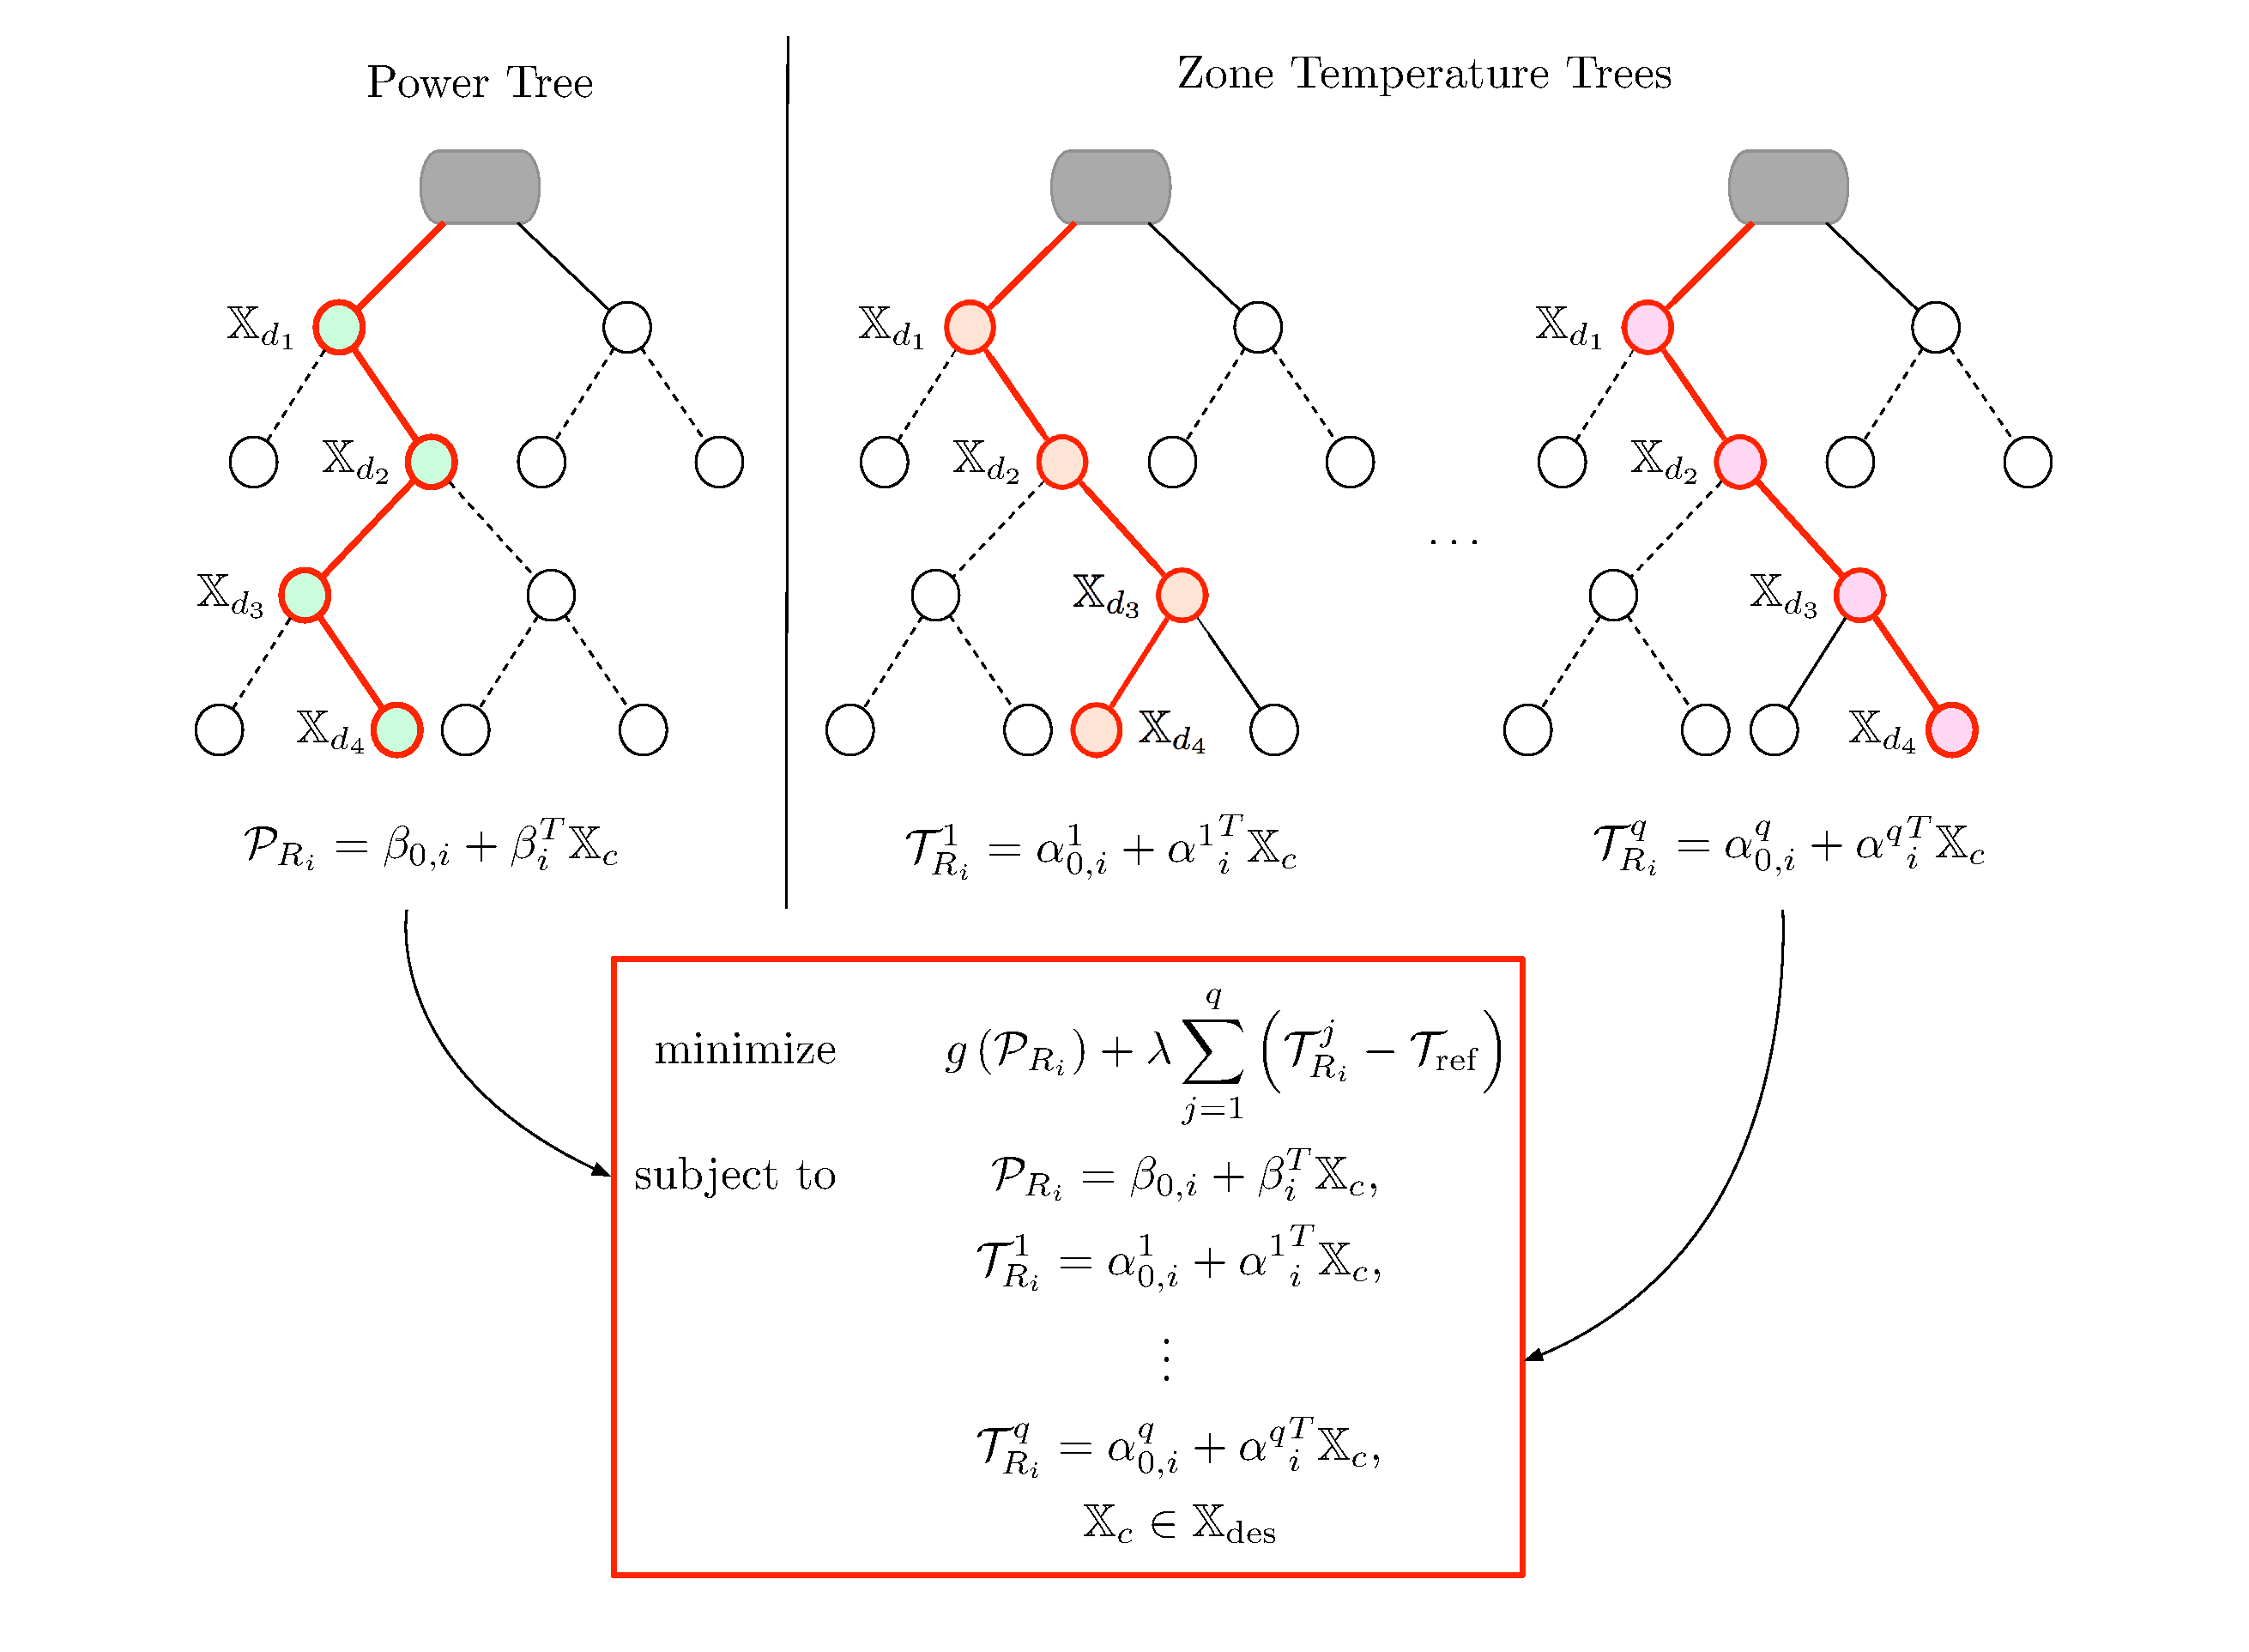
\includegraphics[width=0.95\columnwidth]{Figures/mbCRT.eps}
\caption{DR synthesis with thermal comfort constraints. Each tree is responsible for contributing one constraint to the demand response optimization.}
\label{fig:dropt}
\end{figure}

\subsection{DR synthesis optimization}
In the case of DR synthesis for buildings, the response variable is power consumption, and the objective function can denote the financial reward of minimizing the power consumption during the DR event. However, the curtailment must not result in high levels of discomfort for the building occupants. In order to account for thermal comfort, in addition to learning the tree for power consumption forecast, we can also learn different trees to predict the temperature of different zones in the building. As shown in Fig.~\ref{fig:dropt} and Algo.~\ref{alg:mbcrt}, at each time-step during the DR event, a forecast of the non manipulated variables is used by each tree, to navigate to the appropriate leaf node. For the power forecast tree, the linear model at the leaf node relates the predicted power consumption of the building to the manipulated/control variables, i.e. $\mathcal{P}_{R_i} = \beta_{0,i} + \beta^T_i \mathbb{X}_c$. Similarly, for the $j^{\mathrm{th}}$ zone, a tree is built whose response variable is the zone temperature $\mathcal{T}^j$. The linear model at the leaf node of each of the zone temperature tree relates the predicted zone temperature to the manipulated variables, i.e. $\mathcal{T}_{R_i}^j = \alpha_{0,i}^j + {\alpha^j}^T_i \mathbb{X}_c$.

Therefore, at every time-step, based on the forecast of the non-manipulated variables, we obtain $q+1$ linear models between the power consumption and $q$ zone temperatures and the manipulated variables. We can then solve the following DR synthesis optimization problem to obtain the values of the manipulated variables $\mathbb{X}_c$:

\begin{align}
\begin{aligned}
\text{minimize } \ \ \ & \ \ \ g\left(\mathcal{P}_{R_i}\right) + \lambda \sum_{j=1}^{q} \left( \mathcal{T}^j_{R_i} - \mathcal{T}_{\mathrm{ref}}\right) \\ \text{subject to } \ \ \ &  \ \ \ \ \ \ \mathcal{P}_{R_i} = \beta_{0,i} + \beta^T_i \mathbb{X}_c, \\ \ \ \ & \ \ \ \ \ \mathcal{T}_{R_i}^1 = \alpha_{0,i}^1 + {\alpha^1}^T_i \mathbb{X}_c,  \\ \ \ \ & \ \ \ \ \ \ \ \ \ \ \ \ \ \ \ \ \ \vdots \\ \ \ \ & \ \ \ \ \ \mathcal{T}_{R_i}^q = \alpha_{0,i}^q + {\alpha^q}^T_i \mathbb{X}_c, \\ \ \ \ & \ \ \ \ \ \ \ \ \ \ \ \ \mathbb{X}_c \in \mathbb{X}_{\mathrm{des}}.
  \end{aligned}
\label{eq:synth_program}  
\end{align}
%\begin{center}
%\begin{equation}
%\begin{aligned}
%\underset{\mathbb{X}_c}{\text{minimize}}
% & f(\hat{kW})+\text{Penalty}[\sum_{k=1}^q(\hat{T_k}-T_{ref})] \\
%\text{subject to} \\
%& \hat{kW} = \beta_{0,i} + \beta^T_i \mathbb{X}_c \\
%& \hat{T1} = \alpha_{0,1} + \beta^T_1 \mathbb{X}_c \\
%& \cdots \\
%& \hat{Td} = \alpha_{0,q} + \beta^T_q \mathbb{X}_c \\
%& \mathbb{X}_c \in \mathbb{X}_{safe}
%\end{aligned}
%\label{eq:synth_program}
%\end{equation}
%\end{center}
\begin{figure*}
\centering
  \begin{subfigure}
    \centering
  \includegraphics[width=0.7\columnwidth]{figs/leaf200}
  \end{subfigure}  
  \begin{subfigure}
    \centering
  \includegraphics[width=0.7\columnwidth]{figs/goodleaf}
  \end{subfigure}
%   \subfloat{ \centering \includegraphics[width=\columnwidth]{figs/leaf200}}  
%  \vfil
%  \centering
%   \subfloat{\centering \includegraphics[width=\columnwidth]{figs/goodleaf}}
  \caption{Linear model assumption at the leaves}
  \label{fig:leaf}
\end{figure*}
Here, $\lambda$ is the penalty on the thermal comfort. The linear model between the response variable $\mathcal{P}_{R_i}$ and the control features $\mathbb{X}_c$ is assumed for computational simplicity. Other models could also be used at the leaves as long as they adhere to the separation of variables principle. Fig.~\ref{fig:leaf} shows that the linear model assumption in the leaves of the tree is a valid assumption.

The intuition behind the mbCRT Algo.~\ref{alg:mbcrt} is that at run time $t$, we use the forecast $\mathbb{X}_d(t+1)$ of the disturbance features to determine the leaves of the \textit{controllable} tree and hence, the linear model to be used for the control.
We then solve the simple linear program corresponding to that region to obtain the optimal values of the control variables. 
The mbCRT algorithm is the first ever algorithm which allows the use of regression trees for control synthesis. 


\section{Regression trees with multi-variate output}
\label{S:decision_tree}
Our goal is to construct data-driven functional models that relates the value of the response variable, say power consumption, $\mathcal{P}$ with the values of the predictor variables or features $[\mathbb{X}^1,\dots, \mathbb{X}^n]$ which can include weather data, set-point information and building schedules.
Regression tree based methods are predominantly univariate output, i.e. defined only for single output variable. We describe a splitting criteria for the trees which enables us to predict multiple outputs \cite{StruyfDzeroski2005}. 
If we consider these new outputs as the future states of the single output system, the multi-output tree enables us to implement receding horizon control as the prediction can be made for multiple steps. For example, consider a training dataset with information about the building states like zone temperatures, control set points and ambient weather. The output we are interested in is the power consumption of the building. With a single output model, we can estimate the power consumption of the building at only one time step $T$. The new approach allows us to predict the power consumption of the same building at multiple time steps, i.e. with a tree with $p$ outputs, we can estimate the power consumption at $T, T+1,\dots,T+p$. This is termed as look-ahead capability of a multi-variate output tree. We will consider this example in detail in Sec. \ref{SS:case_dpc}.

In this section, we first explain how a CART based regression tree is built, and then modify it into a multi-variate output model suitable for finite horizon prediction.

\subsection{Model Construction}
\label{SS:training_algo}

We use the following notation. We represent a dataset with $N$ observations, where each input has $n$ features and model has $p$ outputs as
\begin{gather}
x_i := [x_i^1, \dots, x_i^n]^T \in \mathbb{R}^n, \nonumber \\
y_i := [y_i^1, \dots, y_i^p]^T \in \mathbb{R}^p,  \label{E:dataset}\\
i \in \{1,2,\dots, N\}. \nonumber 
\end{gather} 
Splitting of nodes is shown in Fig. \ref{F:RT}. At $i^{\mathrm{th}}$ node, CART splits the data set into 2 subsets. The left branch $R_L$ contains the data corresponding to $x^i \leq t_i$ and the right branch $R_R$ corresponding to $x^i > t_i$. The optimal split at each node is then determined by minimizing the sum of mean square error in both the branches:
\begin{gather}
(x^k,t_k) = \argmin    \sum_{\{i|x_i \in R_L\}}{(y_i - \bar{y}_L)^2}  +  \sum_{\{i|x_i \in R_R\}} {(y_i - \bar{y}_R)^2}
\label{E:CART_split_rule}
\end{gather}
where $y_i \in \mathbb{R}$ and $\bar{y}_L$ and $\bar{y}_R$ are the mean outputs of all the data points in $R_L$ and $R_R$, respectively. The tree is grown in this fashion till the number of data points in the terminal nodes (leaves) exceeds the minimum number of observations in a leaf $minLeaf$, which is often a tuning parameter. Typically a tree is grown till $minLeaf$ size is achieved, and then cost-complexity pruning is employed by collapsing the weak splits \cite{HastieTibshiraniFriedmanEtAl2005}.

\begin{figure}
\centering
\subfigure[First split occurs with input $x^i$ at $t_i$, second split with input $x^j$ at $t_j$ and so on, resulting in 5 regions in this case $R_1, \dots, R_5$.]{
\label{F:RT}
\centering
\begin{tikzpicture}[->,>=stealth',level/.style={sibling distance = 3.5cm/#1,
  level distance = 1.5cm}] 
\node [branch_c] {}
    child[blue!50!gray!,thick]{ node [branch_l] {}
            child[blue!50!gray!,thick]{ node [branch_l] {$R_1$} edge from parent node[above left] {$x^j \leq t_j$}}
            child[red!50!gray!,thick]{ node [branch_r] {$R_2$} edge from parent node[above right] {$x^j > t_j$}} 
            edge from parent node[above left] {$x^i \leq t_i$}                            
    }
    child[red!50!gray!,thick]{ node [branch_r] {}
            child[blue!50!gray!,thick]{ node [branch_l] {}
            		child[blue!50!gray!,thick]{ node [branch_l] {$R_4$} edge from parent node[above left] {$x^k \leq t_k$}}
            		child[red!50!gray!,thick]{ node [branch_r] {$R_5$} edge from parent node[above right] {$x^k > t_k$}} 
            }
            child[red!50!gray!,thick]{ node [branch_r] {$R_3$}}  
            edge from parent node[above right] {$x^i > t_i$}    
		}
; 
\end{tikzpicture}
}
\subfigure[First split occurs with continuous input $x^i$ at $t_i$, second split with categorical input $x^j$ at $t_j^r$ such that $\mathbb{S}_{j,L}=\{ t_j^1,\dots,t_j^r \}$ and $\mathbb{S}_{j,R}=\{ t_j^{r+1},\dots,t_j^q \}$.]{
\label{F:RT2}
\centering
\begin{tikzpicture}[->,>=stealth',level/.style={sibling distance = 3.5cm/#1,
  level distance = 1.5cm}] 
\node [branch_c] {}
    child[blue!50!gray!,thick]{ node [branch_l] {}
            child[blue!50!gray!,dashed,thick]{ node [branch_l] {$R_1$} edge from parent node[above left] {$x^j \in \mathbb{S}_{j,L}$}}
            child[red!50!gray!,dashed,thick]{ node [branch_r] {$R_2$} edge from parent node[above right] {$x^j \in \mathbb{S}_{j,R}$}} 
            edge from parent node[above left] {$x^i \leq t_i$}                            
    }
    child[red!50!gray!,thick]{ node [branch_r] {}
            child[blue!50!gray!,thick]{ node [branch_l] {}
            		child[blue!50!gray!,thick]{ node [branch_l] {$R_4$} edge from parent node[above left] {$x^k \leq t_k$}}
            		child[red!50!gray!,thick]{ node [branch_r] {$R_5$} edge from parent node[above right] {$x^k > t_k$}} 
            }
            child[red!50!gray!,thick]{ node [branch_r] {$R_3$}}  
            edge from parent node[above right] {$x^i > t_i$}    
		}
; 
\end{tikzpicture}
}
\caption{Tree structures for continuous and mix of discrete and continuous variables.}
\captionsetup{justification=centering}
\end{figure}

We extend the same approach to deal with the multi-output data. In order to determine node splits, we are again interested in calculating the splitting variable $x^k$ and the splitting value $t_k$, but this time we account for errors in all $p$ outputs. Appropriately, we modify \eqref{E:CART_split_rule} as follows:
\begin{gather}
(x^k,t_k) = \argmin    \sum_{\{i|x_i \in R_L\}}{||y_i - \bar{y}_L||}_l^2  +  \sum_{\{i|x_i \in R_R\}} {||y_i - \bar{y}_R||}_l^2.
\label{E:DPC_split_rule}
\end{gather}
In this case, $\bar{y}_L,\bar{y}_R \in \mathbb{R}^p$ and represent the mean of $\forall y_i \in R_L$ and $\forall y_i \in R_R$, respectively. Norm in this optimization criteria can be chosen to $l^1$ norm if we want to minimize the largest absolute error in the outputs or $l^2$ norm which will minimize the sum of squares across all the outputs. Further, we can introduce weights matrix $Q \in \mathbb{R}^{p \times p}$ as other tuning parameter and choose the optimization objective similar to the cost function in Model Predictive Control (MPC):
\begin{gather}
\label{E:DPC_split_rule2}
(x^k,t_k) = \argmin    \sum_{\{i|x_i \in R_L\}}{(y_i - \bar{y}_L)}^TQ{(y_i - \bar{y}_L)}  + \sum_{\{i|x_i \in R_R\}} {(y_i - \bar{y}_R)}^TQ{(y_i - \bar{y}_R)}.
\end{gather}
Both  \eqref{E:DPC_split_rule} and \eqref{E:DPC_split_rule2} can be solved numerically by discretizing the search space of $t_k$ between $max(x^k)$ and $min(x^k)$ calculated across $N$ data points. Finer the resolution $\mathit{res}$, better the accuracy of splits. The terminating condition for growing the tree remains unchanged in \eqref{E:DPC_split_rule} and \eqref{E:DPC_split_rule2}.

So far, we covered how a tree is built when all the features/variables are continuous. it is often the case that some of the features in the data set are categorical, i.e. they can only take discrete values. 
The problem of partitioning a set of discrete values in two subsets is a combinatorial problem. Consider a categorical input feature $x^c$ which can take $q$ different values belonging to the set $\mathbb{S}_c=\{t_c^1,\dots,t_c^q \}$. Number of ways to partition $\mathbb{S}_c$ into two non-empty subsets are $2^{q-1}-1$. Note that the different possible partitions scale exponentially with $q$, unlike in the continuous case where it grows linearly with $res$. Hence, when $q$ is large, exact search is not computationally easy to solve. We use a near-optimal approach to narrow down this search over all possible partitions. The approach is simliar to the one described in \cite{Ripley2007} for single-output system. We first find out all $y_i$s corresponding to each element in $\mathbb{S}_c$ and then order the set $\mathbb{S}_c$ according to an increasing mean:
\begin{gather}
\label{E:DPC_cat_split_rule}
\bar{y}_q = \frac{\displaystyle\sum_{\{i|x^c=t_c^q\}} ||y_i||_l}{N_q},
\end{gather}
where $N_q$ is the number of data points for which $x^c=t_q$. Once $\mathbb{S}_c=\{t_c^1,\dots,t_c^q \}$ is ordered such that 
$\bar{y}_1< \dots < \bar{y}_q$, we split the variable as if it is a continuous variable using \eqref{E:DPC_split_rule} or \eqref{E:DPC_split_rule2} depending upon the chosen type of formulation. If the cost is minimized for $x^c \leq t_c^r$, then the left branch contains $x^c \in \mathbb{S}_{c,L} = \{ t_c^1,\dots,t_c^r \}$ and the right branch contains $x^c \in \mathbb{S}_{c,R} = \{ t_c^{r+1},\dots,t_c^q \}$. A tree with a mix of continuous and categorical variables is shown in Fig. \ref{F:RT2}. 

%\begin{figure}
%\centering
%\begin{tikzpicture}[->,>=stealth',level/.style={sibling distance = 3.5cm/#1,
%  level distance = 1.5cm}] 
%\node [branch_c] {}
%    child[blue!50!gray!,thick]{ node [branch_l] {}
%            child[blue!50!gray!,dashed,thick]{ node [branch_l] {$R_1$} edge from parent node[above left] {$x^j \in \mathbb{S}_{j,L}$}}
%            child[red!50!gray!,dashed,thick]{ node [branch_r] {$R_2$} edge from parent node[above right] {$x^j \in \mathbb{S}_{j,R}$}} 
%            edge from parent node[above left] {$x^i \leq t_i$}                            
%    }
%    child[red!50!gray!,thick]{ node [branch_r] {}
%            child[blue!50!gray!,thick]{ node [branch_l] {}
%            		child[blue!50!gray!,thick]{ node [branch_l] {$R_4$} edge from parent node[above left] {$x^k \leq t_k$}}
%            		child[red!50!gray!,thick]{ node [branch_r] {$R_5$} edge from parent node[above right] {$x^k > t_k$}} 
%            }
%            child[red!50!gray!,thick]{ node [branch_r] {$R_3$}}  
%            edge from parent node[above right] {$x^i > t_i$}    
%		}
%; 
%\end{tikzpicture}
%\caption{Binary regression tree: first split occurs with continuous input $x^i$ at $t_i$, second split with categorical input $x^j$ at $t_j^r$ such that $\mathbb{S}_{j,L}=\{ t_j^1,\dots,t_j^r \}$ and $\mathbb{S}_{j,R}=\{ t_j^{r+1},\dots,t_j^q \}$.}
%\captionsetup{justification=centering}
%\label{F:RT2}
%\end{figure}

In summary, when the data set contains both types of variables- continuous and categorical, first the range of all the categorical variables is sorted. 
Then, the optimal cost of splitting is determined for each input feature. 
Finally, the input feature for which this cost is minimum is taken as the splitting variable. Following this approach, we obtain a tree model in the form of
\begin{gather}
\begin{pmatrix}
  y^1 \\
  \vdots \\
  y^p 
 \end{pmatrix}
 = \mathit{f} \left( x^1, \dots, x^n \right).
 \label{E:regtree_multi}
\end{gather}

In the context of a building model, this approach is validated in Sec. \ref{SS:performance_test}.

%\subsection{Interpretability of regression trees}
%Regression trees based approaches are our choice of data-driven models since they highly interpretable, by design.
%Interpretability is a fundamental desirable quality in any predictive model.  
%Complex predictive models like neural-networks , support vector regression etc. go through a long calculation routine and involve too many factors. 
%It is not easy for a human engineer to judge if the operation/decision is correct or not or how it was generated in the first place. 
%Building operators are used to operating a system with fixed logic and rules. 
%They tend to prefer models that are more transparent, where it is clear exactly which factors were used to make a particular prediction.
%At each node in a regression tree a simple, if this then that, human readable, plain text rule is applied to generate a prediction at the leafs, which anyone can easily understand and interpret.
%Making machine learning algorithms more interpretable is an active area of research~\cite{giraud1998beyond}, one that is essential for incorporating human centric models in cyber-physical energy systems.

\subsection{Model Validation: Multi-variate outputs}
\label{SS:performance_test}
For a tree with order of autoregression $\delta = 6$ and a prediction horizon $p = 20$ and $Q$ in \eqref{E:DPC_split_rule2} as Identity matrix, the results on the test dataset are shown in Fig. \ref{F:perf_test}. The test set shows a day from July 2013, which the model has never seen before. It shows the building power consumption predicted at any time $\mathcal{P}_T$ as compared to the actual power consumption of the building. Since we can predict the power for multiple steps (horizon) at a time, we compare it to $\mathcal{P}_{T+10}$ calculated 10 steps before $T$, i.e. $T-10$,  $\mathcal{P}_{T+20}$ calculated 20 steps before $T$, i.e. $T-20$, and the ground truth from the test dataset. It can be seen that even with a relatively long horizon, the multi-variate output tree model captures the rapid changes in the response variable (power consumption) very accurately.

\section{Data predictive control} 
\label{S:control_tree}
The data-driven algorithm described so far uses the forecast of features to obtain building power consumption predictions. 
In this section, we describe a control algorithm which utilizes the multi-variate output capability of our regression tree model to implement receding horizon control. This is also one of our primary contributions.

%Recall that the objective of learning a regression tree is to learn a model $f$ for predicting the response $\mathbb{Y}$ with the values of the predictor variables or features $\mathbb{X}^1, \dots, \mathbb{X}^n$; i.e. $Y=f(\mathbb{X}^1, \dots, \mathbb{X}^n)$.
%Given a forecast of the features $\hat{X}^1, \dots, \hat{X}^n$ we can predict the response $\hat{Y}$. 
%Now consider the case where a subset, $\mathbb{X}_c \subset \mathbb{X}$ of the set of features/variables $\mathbb{X}$'s are manipulated variables i.e. we can change their values in order to drive the response $\mathbb{Y}$ towards a certain value. 
%In the case of buildings, the set of  variables can be separated into disturbances (or non-manipulated) variables like outside air temperature, humidity, wind etc. while the controllable (or manipulated) variables would be the temperature and lighting set-points within the building.
%Our goal is to modify the regression trees and make them suitable for synthesizing the optimal values of the control variables in real-time.
In Sec.~\ref{sec:drsyn} an algorithm for model based control with regression trees (mbCRT) \cite{BehlJainMangharam2016,Behl201630} was presented. This algorithm utilizes a \emph{separation of variables} principle to allow for a control optimization in the leaves of the tree. 
Although mbCRT enables control with regression trees based models, it suffers from two significant limitations:
\begin{enumerate}
\item mbCRT is based on uni-variate output regression tree models and is unable to make multi-variate predictions. 
\item The mbCRT algorithm is a `one-step look-ahead' algorithm. It can only account for an unexpected disturbance only one time-step before it occurs, thus making it sub-par as compared to receding horizon control algorithms.
\end{enumerate}

\begin{figure}
\centering
\includegraphics[scale=0.85]{Figures/receding_horizon.pdf}
\caption{Finite-horizon moving window of MPC: at time $t$, the MPC optimization problem is solved for a finite length window of $N$ steps and the first control input $u(t)$ is applied; the window then recedes one step forward and the process is repeated at time $t+1$.}
\captionsetup{justification=centering}
\label{F:MPC-illust}
\end{figure} 

%In mbCRT, given building data $(\mathbb{X},\mathbb{Y})$ in the form of \eqref{E:dataset}, we can separate the controllable $\mathbb{X}_c$ (or manipulated variables) and uncontrollable variables $\mathbb{X}_d$ (or non-manipulated variables or disturbances) in the features such that $\mathbb{X}_c \cup \mathbb{X}_d \equiv \mathbb{X}$. 
%This is called separation of variables.
%Applying this separation of variables, the regression tree is built only on the non-manipulated variables or disturbances $(\mathbb{X}_d,\mathbb{Y})$.  
%We obtain a model in the following form:
%\begin{gather}
%\mathbb{Y} = \mathit{f} \left( \mathbb{X}^1_d,\dots,\mathbb{X}^n_d \right).
%\label{E:train_model_single}
%\end{gather}
%In the leaf $R_i$ of the tree, we fit a parametric model (linear regression) which is a function only of the controllable/manipulated variables:
%\begin{gather}
%\mathbb{Y}_{R_i} = \beta_{0,i} + \beta^T_i \mathbb{X}_c.
%\end{gather}
%In this manner, we train a regression tree using only $\mathbb{X}_d$, and then in each leaf we train a linear model which is a function only of $\mathbb{X}_d$. 
%To solve the control problem when only $\mathbb{X}_d$ is known, we navigate to an appropriate leaf $R_i$ and determine $\mathbb{X}_c$ from the following optimization problem:
%\begin{align}
%\begin{aligned}
%\text{minimize } \ \ \ & \ \ \ \ \ \ \mathit{g} \left( \mathbb{Y}_{R_i}, \mathbb{X}_c  \right) \\ \text{subject to } \ \ \ & \mathbb{Y}_{R_i} = \beta_{0,i} + \beta^T_i \mathbb{X}_c, \\ \ \ \ & \ \ \ \ \ \ \mathbb{X}_c \in \mathbb{X}_{\mathrm{des}},
%  \end{aligned}
%  \label{E:opt_single}
%\end{align}
%where $g$ is some function of the response variable and/or control variables we wish to minimize.

The finite receding horizon control approach involves optimizing a cost function subject to the dynamics of the system and the constraints, over a finite horizon of time. 
After an optimal sequence of control inputs are computed, the first input is applied, then at the next step the optimization is solved again as shown in Fig. \ref{F:MPC-illust}. 

In the following section, we extend the mbCRT algorithm such that we can implement receding horizon control and address the limitations in mbCRT.  
This algorithm is called data predictive control with regression trees (DPCRT).

\begin{algorithm}[t]
\caption{DPCRT: Data Predictive Control with Regression Trees}
\label{A:DPC}
\begin{algorithmic}[]
\State \textsc{Design Time}
\Procedure{Model Training using Separation of Variables}{}
\State Set $\mathbb{X}_c$ $\gets$ manipulated features
\State Set $\mathbb{X}_d$ $\gets$ non-manipulated features
\State Build predictive tree(s) $\mathfrak{T}$(s) with $(\mathbb{Y},\mathbb{X}_d)$ using \eqref{E:regtree_multi}
\ForAll{regions $R_i$ at the leaves of $\mathfrak{T}$}
\State Choose a function $h$ for the problem
\State Fit linear model $\mathit{h} \left( \mathbb{Y}_{R_i}^1, \dots, \mathbb{Y}_{R_i}^p \right) = \beta_{0,i} + \beta^T_i \mathbb{X}_c$
\EndFor
\EndProcedure
\State \textsc{Run Time}
\Procedure{Predictive Control}{}
\While{$t< t_{\mathrm{stop}}$}
\State Determine the leaf and region $R_{i}(t)$ using $\mathbb{X}_d(t)$
\State Obtain the linear model at $R_{i}(t)$
\State Choose a cost function $g$ for the problem
\State Solve optimization in \eqref{E:opt_multi} or \eqref{E:opt_multi2} to determine optimal control action $\left[\mathbb{X}^*_c(t),\dots,\mathbb{X}^*_c(t+p)\right]^T $
\State Apply the first input $\mathbb{X}^*_c(t)$
\EndWhile
\EndProcedure
\end{algorithmic}
\end{algorithm}

\begin{figure*}[b!]
\centering
\includegraphics[width=0.95\linewidth]{Figures/DPC_tree2.eps}
\caption{Data Predictive Control with Regression Trees with Model Training Process (L) and Receding Horizon Control (R). During control step, the optimal control action $\left[\mathbb{X}^*_c(t),\dots,\mathbb{X}^*_c(t+p)\right]^T $ is determined. The first input $\mathbb{X}^*_c(t)$ is applied to the system. The resulting output $\mathbb{Y}(t)$ which is a feature for the next time step is fed back to determine to determine $R_{i}(t+1)$.}
\captionsetup{justification=centering}
\label{F:DPC_schematic}
\end{figure*}

\subsection{Data predictive control with Regression Trees}
\label{SS:control_algo}

The central idea behind DPCRT is to build a tree model which can also predict future states of the system. Thus, while training a regression tree with multiple response variables, we still use separation of variables as in mbCRT, the difference lies in the number of output variables in each leaf. Therefore, we generate a regression tree of the form
\begin{gather}
\begin{pmatrix}
\mathbb{Y}^1 \\ \vdots \\ \mathbb{Y}^p
\end{pmatrix}
 = \mathit{f} \left( \mathbb{X}^1_d,\dots,\mathbb{X}^n_d \right).
\label{E:train_model_multi}
\end{gather}
In each leaf of the tree, we now fit a linear model on a function $h : \mathbb{R}^p \to \mathbb{R}$ of all the response variables such that
\begin{gather}
\mathit{h} \left( \mathbb{Y}_{R_i}^1, \dots, \mathbb{Y}_{R_i}^p \right) = \beta_{0,i} + \beta^T_i \mathbb{X}_c.
\label{E:linear_leaf}
\end{gather}
A simple example of $h$ is an affine function which we will use for our case study in Sec. \ref{SS:case_dpc}. Once the model is trained, we solve the following optimization problem:
\begin{align}
\begin{aligned}
\text{minimize } \ \ \ & \ \ \ \ \ \ \ \ \ \ \ \ \ \ \ \mathit{g} \left( h, \mathbb{X}_c  \right) \\ \text{subject to } \ \ \ & \mathit{h} \left( \mathbb{Y}_{R_i}^1, \dots, \mathbb{Y}_{R_i}^p \right) = \beta_{0,i} + \beta^T_i \mathbb{X}_c, \\ \ \ \ & \ \ \ \ \ \ \ \ \ \ \ \ \ \ \ \mathbb{X}_c \in \mathbb{X}_{\mathrm{des}}.
  \end{aligned}
  \label{E:opt_multi}
\end{align}

We solve this optimization in the same manner as finite receding horizon control, and $\mathbb{X}_c$ includes all the control variables for the chosen horizon, i.e. $\mathbb{X}_c := \left[\mathbb{X}_c(t), \dots, \mathbb{X}_c(t+p)\right]^T$. We choose the first optimal control input $\mathbb{X}_c^*(t)$ and proceed to the next time step.

If the number of control variables is large, the optimization problem \eqref{E:opt_multi} may require many data points in the leaves or in other words a large $minLeaf$ which can affect the accuracy of the regression tree. 
Therefore, we also introduce a variant of this algorithm which will ease the selection of a lower $minLeaf$:
\begin{align}
\begin{aligned}
\text{minimize } \ \ \ & \ \ \ \ \ \ \ \ \ \mathit{g} \left( h^1, \dots, h^{\mathrm{nc}}, \mathbb{X}_c  \right) \\ \text{subject to } \ \ \ & \mathit{h}^1 \left( \mathbb{Y}_{R_i}^1, \dots, \mathbb{Y}_{R_i}^p \right) = \beta_{0,i} + \beta^T_i \mathbb{X}_c^1, \\ \ \ \ & \ \ \ \ \ \ \ \ \ \ \ \ \ \ \ \ \ \ \vdots \\ \ \ \ & \mathit{h}^{\mathrm{nc}} \left( \mathbb{Y}_{R_i}^1, \dots, \mathbb{Y}_{R_i}^p \right) = \gamma_{0,i} + \gamma^T_i \mathbb{X}_c^{\mathrm{nc}}, \\ \ \ \ & \ \ \ \ \ \ \ \ \ \ \ \ \ \ \ \mathbb{X}_c \in \mathbb{X}_{\mathrm{des}}.
  \end{aligned}
  \label{E:opt_multi2}
\end{align}


Here, $h^j$ is a linear model which depends only in the control variable $\mathbb{X}_c^j$. Note that $\mathbb{X}_c^j$ can still be a vector when horizon length is greater than 1. With suitable choice of $g$ and $h$, the problems \eqref{E:opt_multi} and \eqref{E:opt_multi2} can be formed as convex optimization problems. 

Our algorithm for DPC with regression trees in summarized in Algo. \ref{A:DPC} and a schematic is shown in Fig. \ref{F:DPC_schematic}. During training process, the tree is trained only on uncontrollable variables with linear models in the leaves which are a function only of controllable variables. During the control step, at time $t$, the uncontrollable features $\mathbb{X}_d(t)$ are known and thus the leaf $R_{i}(t)$ is known. The optimization problem in $R_i(t)$ is solved to determine the control action $\left[\mathbb{X}^*_c(t),\dots,\mathbb{X}^*_c(t+p)\right]^T $. The first input $\mathbb{X}^*_c(t)$ is applied to the system. The resulting output $\mathbb{Y}(t)$ which is a feature for the next time step is fed back to determine to determine $R_{i}(t+1)$.
In the context of a building model, we show the efficacy of DPCRT in Sec. \ref{SS:DPC_model_validation}.

\subsection{Model Validation: DPCRT}
\label{SS:DPC_model_validation}

\begin{figure}
\subfigure[Building power consumption at time $T$ predicted at time $T$ is denoted by $\mathcal{P}_{T}$, predicted 10 steps ahead at time $T-10$ is denoted by $\mathcal{P}_{T+10}$, and predicted 20 steps ahead at time $T-20$ is denoted by $\mathcal{P}_{T+20}$]{
\centering
\includegraphics[width=18pc]{Figures/perf_test.eps}
\label{F:perf_test}
}
\subfigure[A comparison of power consumption of the building for two different regression trees. $\mathcal{T}_1$ is trained on all the features while $\mathcal{T}_2$ is trained only on non-manipulated features using separation of variables.]{
\centering
\includegraphics[width=18pc]{Figures/separation_vars.eps}
\label{F:separation_vars}
}
\subfigure[Model validation for linear regression at the leaves of the tree. The predicted and the actual power consumption are very close.]{
\label{F:linear_approx2}
\centering
\includegraphics[width=18pc]{Figures/error_leaf2_1.eps}
}
\subfigure[The tree has 703 leaves. For each leaf, a maximum and a minimum error in prediction of average power consumption over the control horizon $\mathcal{P}_{\mathrm{pred}}-\mathcal{P}_{\mathrm{act}}$ is calculated from the data points that end up in that leaf.]{
\centering
\includegraphics[width=18pc]{Figures/error_leaf.eps}
\captionsetup{justification=centering}
\label{F:linear_approx}
}
\caption{Model Validation of DPCRT.}
\captionsetup{justification=centering}
\end{figure}

The performance of DPCRT depends on two key assumptions: (a) first, is that the separation of variables doesn't introduce significant errors while training the tree, and (b) second, that the linear regression at the leaves is a valid assumption.
We verify the validity of these assumptions in terms of their effect on model accuracy.

\subsubsection{Separation of Variables}
We train two kinds of regression trees: (1) a tree $\mathcal{T}_1$ that has all the features as described earlier, and (2) a tree $\mathcal{T}_2$ that was learned from non-manipulated variables only with a linear model on the control/manipulated variables at the leaves.
%These 3 features are considered to be the control variables. 
%In other words, $\mathcal{T}_1$ is trained on all the features $\mathbb{X}$ while $\mathcal{T}_2$ is trained only on non-manipulated features $\mathbb{X}_d$. 
The predicted power consumption of the building at time $T$ and $T+5$ (see \eqref{E:building_model}), i.e. $\mathcal{P}_T$ and $\mathcal{P}_{T+5}$, respectively, for both trees is shown in Fig. \ref{F:separation_vars}. The normalized root mean square error (NRMSE) for these 2 outputs on the test dataset is shown in Tab. \ref{T:NMRSE_separation_vars}. We notice a small loss in model accuracy with $\mathcal{T}_2$ due to the separation of variables. 
This is the opportunity cost for integrating control synthesis with the tree, since otherwise the control features would have been a part of the splitting criteria rather than a linear model in the leaves of the tree.
%As seen in Fig. \ref{F:separation_vars} and Tab. \ref{T:NMRSE_separation_vars}, this error is not significant. 
In the case of $\mathcal{T}_2$ we exploit the tree structure to reach the right leaf, the actual output is determined by fitting a linear model which is a function of the controlled variables.

\begin{table}
  \centering
  \caption{NRMSE for regression trees with $(\mathcal{T}_1)$ and without $(\mathcal{T}_2)$ controllable features.}
    \begin{tabular}{c|c|c|c|c|c|c}
    \toprule
     & $\mathcal{P}_{T}$ &$\mathcal{P}_{T+1}$ &$\mathcal{P}_{T+2}$ &$\mathcal{P}_{T+3}$ &$\mathcal{P}_{T+4}$ & $\mathcal{P}_{T+5}$ \\
    \midrule
    $\mathcal{T}_1$     & 0.1037  &  0.1036 &   0.1116 &   0.1124 &   0.1140  &  0.1164  \\
    $\mathcal{T}_2$     & 0.1156  &  0.1182 &   0.1270 &   0.1268 &   0.1324  &  0.1308  \\
    \bottomrule
    \end{tabular}
  \label{T:NMRSE_separation_vars}
\end{table}

\subsubsection{Linear Approximation at Leaves}
For the tree $\mathcal{T}_2$, we fit a linear model on the sum of all outputs, i.e. the sum of power consumption over the complete control horizon. Recall \eqref{E:linear_leaf} which is now expressed as
\begin{gather}
\mathbb{Y}_{R_i}^1+ \dots + \mathbb{Y}_{R_i}^p  = \beta_{0,i} + \beta^T_i \mathbb{X}_c.
\end{gather}
Equivalently,in terms on power consumption, at each leaf we fit a linear model:
\begin{gather}
\mathcal{P}_{T}+ \dots + \mathcal{P}_{T+p}  = \beta_{0} + \beta^T \mathbb{X}_c.
\end{gather}
%\begin{figure}
%\centering
%\includegraphics[width=20pc]{Figures/error_leaf.eps}
%\caption{The tree has 703 leaves. For each leaf, a maximum and a minimum error in prediction of average power consumption over the control horizon $\mathcal{P}_{\mathrm{pred}}-\mathcal{P}_{\mathrm{act}}$ is calculated from the data points that end up in that leaf. }
%\captionsetup{justification=centering}
%\label{F:linear_approx}
%\end{figure}
For 2 randomly selected leaves, the fit of the linear model against the actual power consumption is shown in Fig. \ref{F:linear_approx2}. The error observed in the predicted and actual power consumption for all leaves is depicted in Fig. \ref{F:linear_approx}.
It can be seen that for a small number of samples in the leaves of the tree the linear model assumption is valid.



\section{Case Study}
\label{sec:case}
%\begin{figure}
%\centering
%\includegraphics[width=\columnwidth]{matlab.jpg}
%  \caption{DR-Advisor toolbox for power, price, weather and schedule data capture, baseline prediction, DR policy evaluation and DR synthesis}
%  \label{gui}
%\end{figure}

%DR-Advisor (Figure~\ref{gui}) has been developed into a MATLAB toolbox available at \url{http://mlab.seas.upenn.edu/dr-advisor/}.
In this section, we present a comprehensive case study to show how DR-Advisor can be used to address all the aforementioned demand response challenges (Sec.~\ref{sec:problem}) and we compare the performance of our tool with other data-driven methods. 

\begin{figure}
\centering
\includegraphics[width=0.8\columnwidth]{figs/penn-compressed}
\caption{8 different buildings on Penn campus were modeled with DR-Advisor}
\label{fig:penn}
\end{figure}

\subsection{Building description}
We use historical weather and power consumption data from 8 buildings on the Penn campus (Fig.~\ref{fig:penn}). These buildings are a mix of scientific research labs, administrative buildings, office buildings with lecture halls and bio-medical research facilities. The total floor area of the eight buildings is over 1.2 million square feet spanned across. The size of each building is shown in Tab.~\ref{tab:penn}.

We also use the DoE Commercial Reference Building (DoE CRB) simulated in EnergyPlus as the virtual test-bed building.
This is a large 12 story office building consisting of 73 zones with a total area of 500,000 sq ft. 
There are 2397 people in the building during peak occupancy. 
During peak load conditions the building can consume up to 1.6 MW of power. 
For the simulation of the DoE CRB building we use actual meteorological year data from Chicago for the years 2012 and 2013. 
On July 17, 2013, there was a DR event on the PJM ISO grid from 15:00 to 16:00 hrs. We simulated the DR event for the same interval for the virtual test-bed building.

\subsection{Model Validation}
For each of the Penn buildings, multiple regression trees were trained on weather and power consumption data from August 2013 to  December 2014. 
Only the weather forecasts and proxy variables were used to train the models.
We then use the DR-Advisor to predict the power consumption in the test period \ie for several months in 2015. 
The predictions are obtained for each hour, making it equivalent to baseline power consumption estimate. 
The predictions on the test-set are compared to the actual power consumption of the building during the test-set period. 
%\begin{figure}
%\centering
%\includegraphics[height=3cm, width=\columnwidth]{figs/crbvalid-compressed}
%\caption{Model validation for the clinical research building at Penn.}
%\label{fig:clinical}
%\end{figure}
%One such comparison for the clinical reference building is shown in Figure~\ref{fig:clinical}. 
The following algorithms were evaluated: single regression tree, k-fold cross validated (CV) trees, boosted regression trees (BRT) and random forests (RF).
Our chosen metric of prediction accuracy is the one minus the normalized root mean square error (NRMSE). NRMSE is the RMSE divided by the mean of the data. The accuracy of the model of all the eight buildings is summarized in Tab.~\ref{tab:penn}. We notice that DR-Advisor performs quite well and the accuracy of the baseline model is between 92.8\% to 98.9\% for all the buildings.
\begin{table}
\centering
\caption{Model validation with Penn data.}
%\resizebox{\columnwidth}{!}{%
    \begin{tabular}{l|c|c|c}
    \toprule
    Building Name            & Total Area (sq-ft) & Floors & Accuracy (\%) \\
    \midrule
    LRSM                       & 92,507             & 6      & 94.52       \\
    College Hall               & 110,266            & 6      & 96.40       \\
    Annenberg Center           & 107,200            & 5      & 93.75       \\
    Clinical Research Building & 204,211            & 8      & 98.91       \\
    David Rittenhouse Labs     & 243,484            & 6      & 97.91       \\
    Huntsman Hall              & 320,000            & 9      & 95.03       \\
    Vance Hall                 & 106,506            & 7      & 92.83       \\
    Goddard Labs               & 44,127             & 10     & 95.07   \\
    \bottomrule
    \end{tabular}
 %   }
 \label{tab:penn}   
\end{table}

\subsection{Energy Prediction Benchmarking}
\label{sec:ashrae}
We compare the performance of DR-Advisor with other data-driven method using a bench-marking data-set from the American Society of Heating, Refrigeration and Air Conditioning Engineers (ASHRAE's) Great Energy Predictor Shootout Challenge~\cite{kreider1994predicting}. 
The goal of the ASHRAE challenge  was to explore and evaluate data-driven models that may not have such a strong physical basis, yet that perform well at prediction.
%The competition attracted $\sim150$ entrants, who attempted to predict the unseen power loads from weather and solar radiation data using a variety of approaches.
In addition to predicting the hourly whole building electricity consumption, WBE (kW), both the hourly chilled water, CHW (millions of Btu/hr) and hot water consumption, HW (millions of Btu/hr) of the building was also required to be a prediction output. Four months of training data with the following features was provided: 
\begin{inparaenum}(a)
\item Outside temperature ($^\circ$F)
\item Wind speed (mph)
\item Humidity ratio (water/dry air)
\item Solar flux (W/$m^2$)
\end{inparaenum}
In addition to these training features, we added three proxy variables of our own: hour of day, IsWeekend and IsHoliday to account for correlation of the building outputs with schedule. 

\begin{table}[b!]
\centering
\caption{ASHRAE Energy Prediction Competition Results.}
%\resizebox{\columnwidth}{!}{%
    \begin{tabular}{c|c|c|c|c}
    \toprule
    ASHRAE Team ID & WBE CV & CHW CV & HW CV & Average CV \\
    \midrule
    9              & 10.36  & 13.02  & 15.24 & 12.87      \\
    \textbf{DR-Advisor} & \textbf{11.72}  & \textbf{14.88}  & \textbf{28.13} & \textbf{18.24}     \\
    6              & 11.78  & 12.97  & 30.63 & 18.46      \\ 
    3              & 12.79  & 12.78  & 30.98 & 18.85      \\
    2              & 11.89  & 13.69  & 31.65 & 19.08      \\
    7              & 13.81  & 13.63  & 30.57 & 19.34      \\
    \bottomrule
    \end{tabular}
  %  }
    \label{tab:results}
\end{table}

We use different ensemble methods within DR-Advisor to learn models for predicting the three different building attributes. 
In the competition, the winners were selected based on the accuracy of all predictions as measured by coefficient of variation (CV) statistic. 
The smaller the value of CV, the better the prediction accuracy.
ASHRAE released the results of the competition for the top 19 entries which they received. 
In Tab.~\ref{tab:results}, we list the performance of the top 5 winners of the competition and compare our results with them.
It can be seen from Tab.~\ref{tab:results}, that the random forest implementation in the DR-Advisor tool ranks $2^{nd}$ in terms of WBE CV and the overall average CV. 
%The winner of the competition was an entry from David Mackay~\cite{mackay1994bayesian} which used a particular form of bayesian modeling using neural networks.

The result we obtain clearly demonstrates that the regression tree based approach within DR-Advisor can generate predictive performance that is comparable with the ASHRAE competition winners. 
%Furthermore, since regression trees are much more interpretable than neural networks, their use for building electricity prediction is, indeed, very promising.

\begin{figure}
\subfigure[Rule-based strategies used in DR Evaluation. CHSTP denotes Chiller set point and CLGSTP denotes Zone Cooling temperature set point.]{
\includegraphics[height=6cm, width=0.5\columnwidth]{figs/ControlStrategy-compressed}
\label{fig:case_eval_control}
 }
\subfigure[Prediction of power consumption for 3 strategies. DR Evaluation shows that Strategy 1 (S1) leads to maximum power curtailment.]{
\label{fig:case_eval_power}
\includegraphics[height=6cm, width=0.5\columnwidth]{figs/PowerOutput-compressed}
}
\caption{DR Evaluation.}
\end{figure}

\subsection{DR-Evaluation}
\label{sec:case_eval}

We test the performance of 3 different rule based strategies shown in Fig. \ref{fig:case_eval_control}. 
%The three strategies differ only during the DR Event. 
Each strategy determines the set point schedules for chiller water, zone temperature and lighting during the DR event. 
These strategies were derived on the basis of automated DR guidelines provided by Siemens~\cite{siemensdr}.
%Cooling set point is same in all three cases. 
Chiller water set point is same in Strategy 1 (S1) and Strategy 3 (S3), higher than that in Strategy 2 (S2). Lighting level in S3 is higher than in S1 and S2.
We use auto-regressive trees (Sec.~\ref{sec:autort}) with order, $\delta = 6$ to predict the power consumption for the entire duration (1 hour) at the start of DR Event. In addition to learning the tree for power consumption, additional auto-regressive trees are also built for predicting the zone temperatures of the building.
At every time step, first the zone temperatures are predicted using the trees for temperature prediction. 
Then the power tree uses this temperature forecast along with lagged power consumption values to predict the power consumption recursively until the end of the prediction horizon.

Fig. \ref{fig:case_eval_power} shows the power consumption prediction using the auto-regressive trees and the ground truth obtained by simulation of the DoE CRB virtual test-bed for each rule-based strategy. 
Based on the predicted response, in this case DR-Advisor chooses to deploy the strategy S1, since it leads to the least amount of electricity consumption. The predicted response due to the chosen strategy aligns well with the ground truth power consumption of the building due to the same strategy, showing that DR strategy evaluation prediction of DR-Advisor is reliable and can be used to choose the best rule-based strategy from a set of pre-determined rule-based DR strategies.

\subsection{DR-Synthesis}
\label{sec:case_syn}

 \begin{figure}
\centering
\includegraphics[width=0.78\columnwidth]{figs/newsynth1-compressed}
\caption{DR synthesis using the mbCRT algorithm for July 17, 2013. A curtailment of $380\si{\kilo\watt}$ is sustained during the DR event period.}
\label{fig:synthesis}
\vspace{-10pt}
\end{figure}

We now evaluate the performance of the mbCRT (Sec.~\ref{sec:mbcrt}) algorithm for real-time DR synthesis. 
%Similar to DR evaluation, the regression tree is trained on weather, proxy features, set-point schedules and data from the building. 
We first partition the set of features into manipulated features (or control inputs) and non-manipulated features (or disturbances). 
There are three control inputs to the system: the chilled water set-point, zone air temperature set-point and lighting levels.
At design time, the model based tree built (Algo.~\ref{alg:mbcrt}) has 369 leaves and each of them has a linear regression model fitted over the control inputs with  the response variable being the power consumption of the building.
In addition to learning the power consumption prediction tree, 19 additional model based trees were also built for predicting the different zone temperatures inside the building.
When the DR event commences, at every time-step (every 5 mins), DR-Advisor uses the mbCRT algorithm to determine which leaf, and therefore, which linear regression model will be used for that time-step to solve the linear program \eqref{eq:synth_program} and determine the optimal values of the control inputs to meet a sustained response while maintaining thermal comfort.
% \begin{figure}
%\centering
%\includegraphics[width=\columnwidth]{figs/setpoints-compressed}
%\caption{Optimal DR strategy as determined by the mbCRT algorithm.}
%\label{fig:set-points}
%\vspace{-10pt}
%\end{figure}
%
%\begin{figure}
%\centering
%\includegraphics[width=\columnwidth]{figs/alltemps-compressed}
%\caption{The mbCRT algorithm maintains the zone temperatures within the specified comfort bounds during the DR event.}
%\label{fig:alltemps}
%\vspace{-10pt}
%\end{figure}

\begin{figure*}[b]
\centering
\subfigure[Optimal strategy using mbCRT.]{
\centering
\includegraphics[width=0.48\textwidth]{figs/setpoints-compressed}
\label{fig:set-points}
} \hspace{2pt}
\subfigure[mbCRT maintains thermal comfort.]{
\centering
\includegraphics[width=0.48\textwidth]{figs/alltemps-compressed}
\label{fig:alltemps}
}
\caption{mbCRT DR control strategy and thermal comfort evaluation.}
\end{figure*}

Fig.~\ref{fig:synthesis} shows the power consumption profile of the building using DR-Advisor for the DR event. 
We can see that using the mbCRT algorithm we are able to achieve a sustained curtailed response of $380\si{\kilo\watt}$ over a period of 1 hour as compared to the baseline power consumption estimate.  Also shown in the figure is the comparison between the best rule based fixed strategy which leads to the most curtailment in Section~\ref{sec:case_eval}. In this case the DR strategy synthesis outperforms the best rule base strategy (from Sec.~\ref{sec:case_eval}, Fig.~\ref{fig:case_eval_power}) by achieving a 17\% higher curtailment while maintaining thermal comfort. The rule-based strategy does not directly account for any effect on thermal comfort.
The DR strategy synthesized by DR-Advisor is shown in Fig.~\ref{fig:set-points}. 
We can see in Fig.~\ref{fig:alltemps} how the mbCRT algorithm is able to maintain the zone temperatures inside the building within the specified comfort bounds.
These results demonstrate the benefit of synthesizing optimal DR strategies as opposed to relying on fixed rules and pre-determined strategies which do not account for any guarantees on thermal comfort. 
Fig.~\ref{fig:model-sel} shows a close of view of the curtailed response. The leaf node which is being used for the power consumption constraint at every time-step is also shown in the plot.
We can see that the model switches several times during the event, based on the forecast of disturbances. 
These results show the effectiveness of the mbCRT algorithm to synthesize DR actions in real-time while utilizing a simple data-driven tree-based model.

\subsubsection{\textbf{Revenue from Demand Response}}
We use Con Edison utility company's commercial demand response tariff structure~\cite{edison} to estimate the financial reward obtained due to the curtailment achieved by the DR-Advisor for our Chicago based DoE commercial reference building.
The utility provides a $\$25/\si{\kilo\watt}$ per month as a reservation incentive to participate in the real-time DR program for summer. A payment of \$1 per kWh of energy curtailed is also paid. For our test-bed, the peak load curtailed is $380\si{\kilo\watt}$. If we consider $\sim$5 such events per month for 4 months, this amounts to a revenue of $\sim$\$45,600 for participating in DR which is 37.9\% of the energy bill of the building for the same duration (\$120,317).
This is a significant amount, especially since using DR-Advisor does not require an investment in building complex modeling or installing sensor retrofits to a building.

\subsection{DPC for Peak Power Reduction}
\label{SS:case_dpc}
We next, evaluate the performance of DPCRT (Sec.~\ref{S:control_tree}) for peak power reduction in buildings. This case study is chosen to reflect the advantages of receding horizon control with regression trees to that on one-step look-ahead control as is performed by mbCRT. 
We compare 2 different control algorithms: mbCRT \cite{BehlJainMangharam2016} and DPCRT for peak power curtailment. Recall the model of the building in Sec. \ref{SS:performance_test}. As described before, the data samples consist of 4 types of features, namely weather data, schedule data, building data and autoregressive terms of building power consumption. Of all the features, we use 3 features from the Building Data as controllable variables. These are 
\begin{enumerate}[leftmargin=0.5cm,topsep=1pt,itemsep=-1ex,partopsep=1ex,parsep=1ex]
\item Zone Temperature Cooling Set Point $\mathcal{C}$ [$^{\circ}$C],
\item Chilled Water Temperature Set Point $\mathcal{H}$ [$^{\circ}$C], and
\item Lighting Set Point $\mathcal{L}$ [-].
\end{enumerate}
%\begin{figure}[t]
%\centering
%\begin{tikzpicture}[node distance = 2cm, auto]
%  \node (vd) at (0,0) {\includegraphics[width=20pc]{Figures/scenario2.png}};
%  \coordinate [label=left:16:00] (v) at (1.0,-2.1);
%  \coordinate [label=left:17:00] (v) at (3.85,-2.1);
%  \coordinate [label=right:15:30] (alpha) at (-1.95,-2.1);  
%  \coordinate [label=right:15:00] (alpha) at (-3.85,-2.1);
%  \coordinate [label=right:Peak disturbance] (alpha) at (-1.8,2.3);
%  \coordinate (P) at (-3.6,0);    
%  \draw (P) node[rotate=90] (N) {Power Consumption};
%  \coordinate (Q) at (3.6,0);    
%  \draw (Q) node[rotate=90] (N) {Electricity Price};
%  \draw[stealth-stealth, thick] (-1.5, 2) -- (0.5, 2);
%  \draw[solid, thick] (0.2, 1.85) -- (1.2, 1.85);
%  \draw[solid, thick] (0.2, -1.25) -- (1.2, -1.25);
%  \coordinate [label=right:$30\times$, color=red] (v) at (0.7,0.3);
%  \draw[stealth-stealth, thick] (0.7, 1.85) -- (0.7, -1.25);
%\end{tikzpicture}
%\caption{The test scenario used in the simulations has a $1.5\times$ peak disturbance between 15:30 and 16:00 hrs. The electricity consumption for this peak is typically heavily penalized and is of the order of $30\times$.}
%\captionsetup{justification=centering}
%\label{F:scenario}
%\end{figure}
To predict the power consumption at a future time instance, we first need to predict the zone temperature at that time because they are used as features in the power tree. To accomplish this, two types of trees are built.
\begin{enumerate}[leftmargin=0.5cm,topsep=1pt,itemsep=-1ex,partopsep=1ex,parsep=1ex]
\item Power tree which predicts the power consumption of the building $\mathcal{P}$ using all the features except the controllable features, and
\item Temperature trees which predict the mean zone temperature of each zone. The tree for the $i^{th}$ zone predicts the temperature $\mathcal{T}_i$ using weather data, schedule data and autoregessive terms of the temperature of that zone.
\end{enumerate}
Both the trees use a linear model at the leaves which is a function solely of the controllable variables.
%In the case of mbCRT, we use the formulation \eqref{E:opt_single}, which uses single output regression trees. 
%The objective function $g$ consists of 2 terms: the cost for the power consumption and the cost for the thermal comfort. A factor $\lambda$ is used to trade-off between the two. The optimal control input $\left[  \mathcal{C}^*, \mathcal{H}^*, \mathcal{L}^*  \right]^T $ is determined by solving the following optimization problem at the leaf.
%\begin{align}
%\begin{aligned}
%\text{minimize } \ \ \ & \ \ \ \ \ \ \mathcal{P} + \lambda \sum_i |\mathcal{T}_i - \mathcal{T}_{\mathrm{ref}}| \\ \text{subject to } \ \ \ & \mathcal{T}_i  = \alpha_{0,i} + \alpha_{1,i}\mathcal{C} + \alpha_{2,i}\mathcal{H} + \alpha_{3,i}\mathcal{L} , \\  \ \ \ & \mathcal{P}  = \beta_{0} + \beta_1\mathcal{C} + \beta_2\mathcal{H} + \beta_3\mathcal{L} \\ \ \ \ & \ \ \ \ \ \ \mathcal{C}_{\mathrm{min}} \leq \mathcal{C} \leq \mathcal{C}_{\mathrm{max}}, \\ \ \ \ & \ \ \ \ \ \ \mathcal{H}_{\mathrm{min}} \leq \mathcal{H} \leq \mathcal{H}_{\mathrm{max}}, \\ \ \ \ & \ \ \ \ \ \ \mathcal{L}_{\mathrm{min}} \leq \mathcal{L} \leq \mathcal{L}_{\mathrm{max}}.
%  \end{aligned}
%  \label{E:mbCRT}
%\end{align}
%
For DPC with Regression Trees (DPCRT), we use the formulation \eqref{E:opt_multi2}. Now the objective function covers the cost for the complete horizon. So the governing optimization problem becomes
\begin{align}
\begin{aligned}
\text{minimize } & \sum_{j=1}^p \frac{\mathcal{P}_{\mathrm{j}}^{\mathcal{C}} + \mathcal{P}_{\mathrm{j}}^{\mathcal{H}} + \mathcal{P}_{\mathrm{j}}^{\mathcal{L}}}{3} +  \lambda \sum_{j=1}^p \sum_i \left| \frac{\mathcal{T}_{\mathrm{ij}}^{\mathcal{C}}+\mathcal{T}_{\mathrm{ij}}^{\mathcal{H}}+\mathcal{T}_{\mathrm{ij}}^{\mathcal{L}}}{3} - \mathcal{T}_{\mathrm{ref}} \right| \\ 
\text{subject to } & \ \ \ \mathcal{T}_{\mathrm{ij}}^{\mathcal{C}}  = \alpha_{\mathrm{0,ij}}^{\mathcal{C}} + \alpha_{\mathrm{1,ij}}^{\mathcal{C}} \mathcal{C}_1 + \dots + \alpha_{\mathrm{p,ij}}^{\mathcal{C}} \mathcal{C}_p , \\
\ \ \ & \ \ \ \mathcal{T}_{\mathrm{ij}}^{\mathcal{H}}  = \alpha_{\mathrm{0,ij}}^{\mathcal{H}} + \alpha_{\mathrm{1,ij}}^{\mathcal{H}} \mathcal{H}_1 + \dots + \alpha_{\mathrm{p,ij}}^{\mathcal{H}} \mathcal{H}_p , \\
\ \ \ & \ \ \ \mathcal{T}_{\mathrm{ij}}^{\mathcal{L}}  = \alpha_{\mathrm{0,ij}}^{\mathcal{L}} + \alpha_{\mathrm{1,ij}}^{\mathcal{L}} \mathcal{L}_1 + \dots + \alpha_{\mathrm{p,ij}}^{\mathcal{L}} \mathcal{L}_p , \\
\ \ \ & \ \ \sum_{j=1}^p\mathcal{P}_{\mathrm{j}}^{\mathcal{C}}  = \beta_{\mathrm{0}}^{\mathcal{C}} + \beta_{\mathrm{1}}^{\mathcal{C}} \mathcal{C}_1 + \dots + \beta_{\mathrm{p}}^{\mathcal{C}} \mathcal{C}_p , \\
\ \ \ & \ \ \sum_{j=1}^p\mathcal{P}_{\mathrm{j}}^{\mathcal{H}}  = \beta_{\mathrm{0}}^{\mathcal{H}} + \beta_{\mathrm{1}}^{\mathcal{H}} \mathcal{H}_1 + \dots + \beta_{\mathrm{p}}^{\mathcal{H}} \mathcal{H}_p , \\
\ \ \ & \ \ \sum_{j=1}^p\mathcal{P}_{\mathrm{j}}^{\mathcal{L}}  = \beta_{\mathrm{0}}^{\mathcal{L}} + \beta_{\mathrm{1}}^{\mathcal{L}} \mathcal{L}_1 + \dots + \beta_{\mathrm{p}}^{\mathcal{L}} \mathcal{L}_p , \\
  \ \ \ \ \ & \ \ \ \ \ \ \ \ \ \ \ \ \ \ \mathcal{C}_{\mathrm{min}} \leq \mathcal{C}_j \leq \mathcal{C}_{\mathrm{max}}, \\ 
  \ \ \ \ \ & \ \ \ \ \ \ \ \ \ \ \ \ \ \ \mathcal{H}_{\mathrm{min}} \leq \mathcal{H}_j \leq \mathcal{H}_{\mathrm{max}}, \\ 
  \ \ \ \ \ & \ \ \ \ \ \ \ \ \ \ \ \ \ \ \mathcal{L}_{\mathrm{min}} \leq \mathcal{L}_j \leq \mathcal{L}_{\mathrm{max}}, \\
    \ \ \ \ \ \ \ & \ \ \ \ \ \ \ \ \ \ \ \ \ \ \ \ \ \ j = \left\lbrace 1, \dots, p \right\rbrace.
  \end{aligned}
  \label{E:DPCRT}
\end{align}
Here, the optimization variables are the control inputs for the complete horizon, i.e. $\left[  \mathcal{C}_1, \dots, \mathcal{C}_p  \right]^T $, $\left[  \mathcal{H}_1, \dots, \mathcal{H}_p  \right]^T $ and $\left[  \mathcal{L}_1, \dots, \mathcal{L}_p  \right]^T $.

We now compare the two algorithms when simulated in closed-loop with the EnergyPlus mode of the building. 
The primary difference between mbCRT and DPCRT is that mbCRT is only a single step look-ahead control algorithm while DPCRT is a receding horizon control algorithm. 
In order to compare the performance of DPCRT, we consider a scenario in which there is a significant disturbance which is only anticipated 30 mins in advance and leads to a sudden increase in zone temperatures in the building. This maybe akin to a sunned spike in occupancy or equipment being witched ON at a brief notice.
\begin{figure*}
\centering
\subfigure[Zoomed in view of mbCRT strategy.]{
\centering
\includegraphics[width=0.48\textwidth]{figs/model_switch-compressed}
%\caption{Zoomed in view of the DR synthesis showing how the mbCRT algorithm selects the appropriate linear model for each time-step based on the forecast of the disturbances.}
\label{fig:model-sel}
} \hspace{1pt}
\subfigure[Peak disturbance between 1530-1600 hrs.]{
\includegraphics[width=0.48\textwidth]{figs/peakpowerplot}
\centering
\label{F:scenario}
}
\caption{Left: mbCRT algorithm selects the appropriate linear model for each time-step based on the forecast of the disturbances. Right: The test scenario used in the DPCRT case study simulations has a $1.5\times$ peak disturbance between 15:30 and 16:00 hrs. }
\vspace{-10pt}
\end{figure*}
Under this scenario, it is important to react to the disturbance in a predictive manner in order to minimize the peak power consumption. 
%We test the algorithms on a scenario when there is an unprecedented disturbance which causes a huge peak in the power consumption. 
This scenario is shown in Fig. \ref{F:scenario}. Between 15:30 and 16:00 hrs, an enormous spike in the power consumption ($1.5\times$) is expected because of a scheduled operation.

\begin{figure}[b!]
\centering
\subfigure[Control strategies.]{
\centering
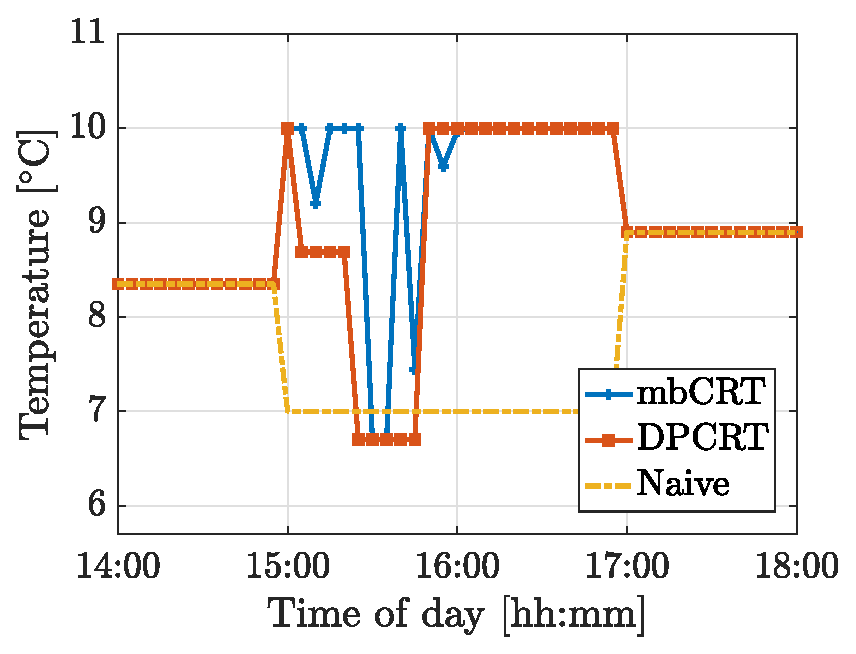
\includegraphics[width=17pc]{Figures/res_control.eps}
\label{F:res_control}
}
\subfigure[Power consumption.]{
\centering
\includegraphics[width=17pc]{Figures/res_power.eps}
\label{F:res_power}
}
\caption{A comparison between mbCRT and DPCRT along with the greedy strategy.}
\captionsetup{justification=centering}
\end{figure}

The control strategies are tested over a 2 hour duration between 15:00 hrs and 17:00 hrs. Fig. \ref{F:res_control} shows 3 control strategies: mbCRT, DPCRT and a Naive load reduction strategy. The naive strategy is equivalent to not responding to the disturbance at all. It maintains the desired zone temeprature set point $\mathcal{C}$, chiller water temperature set point $\mathcal{H}$ and lighting level $\mathcal{L}$ throughout the test period.
In Fig. \ref{F:res_power}, it can be seen that DPCRT reacts to the disturbance much before mbCRT, which waits until the last time-step before the disturbance to react. This leads to a significantly lower peak power consumption that mbCRT.
In the case of DPCRT, the control horizon is 6. 
At 15:00 hrs, DPCRT strategy is same as the greedy one. At 15:05 hrs, the downstream disturbance is visible to DPCRT algorithm and it starts to pre-cool the building by decreasing both cooling and chiller water set points. At 15:25 hrs, the $\mathcal{C}$ and the $\mathcal{H}$ are reduced to mimimum so that in the period of extreme disturbance an optimal trade-off between power consumption and thermal comfort is maintained. Thus, DPCRT algorithm foresees the disturbance and takes a preemptive action against it.  On the other hand, the mbCRT algorithm considers the power consumption and the zone temperatures of only one time step. Therefore, it does not know of an upcoming disturbance. At every time step, it chooses that $\mathcal{C}$, $\mathcal{H}$ and $\mathcal{L}$ which optimizes the cost for that time step. Naturally, this leads to a jaggy behavior in the control strategy.

We can see a similar behavior for the power consumption in Fig. \ref{F:res_power}. The DPCRT algorithm gradually increases the power consumption because it can see the disturbance before it actually reaches 15:30 hrs, while in the case of mbCRT, the power consumption overshoots by a big margin because the controller deals with the disturbance in a single step. DPCRT maintains zone temperature much closer to the reference temperature of 24 degrees while both mbCRT and the naive strategy have large deviations from the desired temperature. 

The quantitative comparison is presented in Tab. \ref{T:case_quant}. Between 15:00 and 17:00 hrs, DPCRT and mbCRT result in similar energy usage, 5102 kWh and 5097 kWh, respectively, both outperforming the Naive strategy which incurs 5358 kWh. Peak power in the case of DPCRT is 1.58 MW which is lower than both mbCRT (1.73 MW) and the Naive strategy (1.63 MW), although Naive outperforms mbCRT. The peak power with DPCRT is 8.6\% less than mbCRT and 3.1\% less than the Naive. While both DPCRT and mbCRT account for thermal comfort, DPCRT deviates less from the desired temperature. The Naive strategy does not trade off on thermal comfort. Thus, DPCRT outperforms mbCRT both in terms of a reduced peak power consumption and better thermal comfort.

%\begin{figure}[t]
%\centering
%\includegraphics[width=20pc]{Figures/res_temp.eps}
%\caption{ Zone temperature of a particular zone under influence of the disturbance.}
%\captionsetup{justification=centering}
%\label{F:res_temp}
%\end{figure}

\begin{table}
  \centering
  \caption{Quantitative comparison for Energy Consumption, Peak Power and \% Reduction in Peak Power of DPCRT compared to Naive approach and mbCRT.}
 % \resizebox{\columnwidth}{!}{
    \begin{tabular}{c|c|c|c}
    \toprule
     & Energy  & Peak Power & Peak \\
     & [kWh] & [MW] & Reduction\\     
    \midrule
    Naive    & 5358  &  1.63 &   3.1\% \\
    mbCRT     & 5097 &  1.73 &   \textbf{8.6\%} \\
    DPCRT     & 5102  &  1.58 &  - \\
    \bottomrule
    \end{tabular}
  %  }
  \label{T:case_quant}
\end{table}


\section{Related Work}
\label{sec:related}
There is a vast amount of literature like (\cite{oldewurtel2013towards,xu2004peak}) which addresses the problem of determining demand response strategies. 
The majority of approaches are using either rule-based approaches for curtailment or white/grey box model-based approaches.
These usually assume that the model of the system is either perfectly known or found in literature, whereas the task is much more complicated and time consuming in case of a real building and sometimes, it can be even more complex and involved than the controller design itself.
After several years of work on using first principles based models for demand response, multiple authors~\cite{costmpc,reallife} have concluded that the biggest hurdle to mass adoption of intelligent building control is the cost and effort required to capture accurate dynamical models of the buildings.
Since DR-Advisor learns an aggregate building level models and combined with the fact that weather forecasts are expected to become cheaper; there is little to no additional sensor cost of implementing the DR-Advisor recommendation system in large buildings. OpenADR standard and protocol~\cite{openadr} describes the formats for information exchange to facilitate DR but modeling, prediction and control strategies are out of scope.
There are ongoing efforts to make tuning and identifying white box models of buildings more autonomous~\cite{new2012autotune}.
Figuring out the correct response on a fast time scales (1-5 mins) using just data-driven methods has'nt been adequately addressed before and makes the DR-Advisor approach and tool novel.

Several machine learning approaches~\cite{edwards2012predicting,vaghefi2014modeling,yin2012scalable} have been utilized before for forecasting electricity load including some which use regression trees. 
However, there are two significant shortcomings of the work in this area: 
\begin{inparaenum}[(a)]
\item First, these approaches are coarse grained and  are not aimed at solving demand response problems but are restricted to long term load forecasting with applications in evaluating building retrofits savings and building energy ratings. 
\item Secondly, there is no focus on control synthesis or addressing the suitability of the model to be used in control design; whereas the mbCRT algorithm enables the use of regression trees for control synthesis with applications in demand response. 
\end{inparaenum}
\label{S:related_work}
There exist several different approaches to balance the power consumption in buildings and avoid peaks, e.g. by load shifting and load shedding \cite{KiliccoteEtAl06aca,LeeEtAl08dom}.
However, they operate on coarse grained time scales and do not guarantee any thermal comfort.
%Another popular approach to energy efficient control for commercial buildings and data centers is model predictive control \cite{MaEtAl10mpc,OldewurtelEtAl10rpe}. %,OldewurtelEtAl10eeb
%In \cite{MaEtAl10mpc} the authors investigated MPC for thermal energy storage in building cooling systems.
%%Stochastic MPC was used to minimize building's energy consumption in \cite{OldewurtelEtAl10eeb}, while 
%Peak electricity demand reduction by MPC with real-time pricing was considered in \cite{OldewurtelEtAl10rpe}.
%These usually assume that the model of the system is either perfectly known or found in literature, whereas the task is much more complicated and time consuming in case of a real building and sometimes, it can be even more complex and involved than the controller design itself.
%After several years of work on using first principles based models for demand response, multiple authors~\cite{costmpc,reallife} have concluded that the biggest hurdle to mass adoption of intelligent building control is the cost and effort required to capture accurate dynamical models of the buildings.

In data-driven optimal control literature, the models are trained on optimal solutions obtained from MPC. The resulting models can then be used for explicit MPC, as in~\cite{BemporadMorariDuaEtAl2002}. This approach has been applied to problems of  stabilization \cite{CavagnariMagniScattolini1999} and freeway traffic systems using regression trees \cite{OleariFrejoCamachoEtAl2015}. 
Another class of methods solve nonlinear optimization directly on the trained models to do receding horizon control. This has been done for wind turbine control using evolutionary optimization algorithm \cite{KusiakSongZheng2009}, and for building control using branch and bound search algorithm \cite{FerreiraRuanoSilvaEtAl2012}. 

%Lastly, MPC like cost function can also be used to find weights in the neural networks. This has been demonstrated in \cite{AkessonToivonen2006}. If the NN models are accurate enough, optimal control can offer a good performance, but this comes at an expense of (a) loss in interpretability, and often (b) computationally complexity because the optimization problem is not convex or/and there is a state space explosion.

%Regression trees on the other hand are highly interpretable. In the case of buildings and many other applications, it is important that the models are easily understandable by the facility managers. It helps them to explain why a particular control strategy is chosen, for example. As we have already seen, 
The DPCRT algorithm is first of its kind that does finite receding horizon control with regression trees. 
It is computationally efficient because the optimization problem is convex and the number of constraints scales linearly with the number of control variables. 
%Its simplicity together with accuracy is unmatched to any other algorithm mentioned above.

\section{Conclusion}
\label{sec:discussion}
\textcolor[rgb]{1.00,0.00,0.00}{We present a data-driven approach for control-oriented modeling of large-scale cyber-physical systems. We show how regression trees are well suited to address challenges associated with Demand-Response for large \textit{C/I/I} consumers while being interpretable. We present a data-driven predictive control with regression trees (DPCRT): an algorithm for implementing receding horizon control with regression trees-based models. DPCRT enables the use of receding horizon control synthesis for complex problems, which otherwise are dependent on first principles based models. We applied DPCRT to the peak power reduction problem in buildings. The performance of DPCRT are evaluated on a DoE commercial reference virtual test-bed. It results in a much lower energy consumption when compared to the Naive control strategy. DPCRT also leads to $8.6\%$ decrease in the peak power reduction of the building when compared to mbCRT and $3.1\%$ when compared to the Naive peak reduction strategy. These advantages combined with the fact that the tree-based methods achieve high prediction accuracy, make DPCRT an alluring tool for evaluating and planning DR curtailment responses for large scale cyber-physical energy systems.}

\textcolor[rgb]{0.00,0.00,1.00}{\textbf{\emph{On-going work.}} The approach we propose in this paper modifies the CART algorithm considering the error minimization of the system evolution over a predictive horizon. This results in a multi-output regression tree-based system modeling that is extremely simple from the computational complexity point of view and that give good accuracy for the prediction. New methodologies are currently under investigation that consider multiple trees with single output. Preliminary results can be found in \cite{JainACC2017,JainCDC2017}.}



%\let\secfnt\undefined
%\newfont{\secfnt}{ptmb8t at 10pt}

\bibliographystyle{abbrv}
\bibliography{references,ref_buildsys,newrefs}

\end{document}


